\chapter{Methods and Implementation}\label{cha:Method}

% längsta avsnittet i rapporten. Den består av en redogörelse av ditt arbete och den visar hur du kommer fram till dina resultat.

% Undvik egna synpunkter. Dessa framförs i Inledningskapitlet och Diskussions-kapitlet

% Ange källa till figurer i slutet. T.ex.  Source: Expedition Mondial.

% Metoddelen beskriver tillvägagångssättet – intervjuer, observationer, litteraturstudier, laborationer och så vidare. Motivera varför en viss metod valdes och vilka eventuella svårigheter som har förekommit. Metoden ska vara replikerbar, vilket innebär att en annan skribent ska kunna göra om studien med hjälp av informationen i metoddelen. Det finns en mängd böcker om olika vetenskapliga metoder. Till exempel kan en intervju utföras på en mängd olika sätt. I rapporter inom humaniora brukar metoddelen vara mer utförlig än i en teknisk rapport.

This chapter presents the methodological framework, via presenting methods to design for learning and motivation.

Then, the setting and research context is described, together with a description of the participants.

Then, application implementation is described, followed by presenting the study design and data collection.

The final topic is data analysis theory.

\section{Methodological framework}

\subsection{Methods to Design for Learning}

%\citep{effectivelearning-robert}
%\citep{learning-krathwohl}
%\citep{learning-ucla}

The following sections, are about how to design for effective learning, by designing for the mind, cognitive psychology.

Cognitive psychology deals with how our brain works in regards to our memory.

The section presents strategies and techniques to design learning for the mind, and what needs to be considered.

Two aspects are especially relevant when it comes to education: how humans learn (the first four sections), and how humans forget (the two last sections).

In how humans learn, the purpose is to find the most powerful strategies and techniques to design effective learning (mapping educational objectives, how to build skills, pattern-matching techniques, and the power of reflection and assessing).

In how people forget, UCLA Bjork's Learning and Forgetting Lab \cite{ucla} researches how people forget, and how to design so that people do not forget ( retrieval practice and spaced practice).

%On January 28th, 2016, Henrik Marklund\ref{effectivelearning-expert} at the educautional technology startup Knowly was interviewed about Pedagogic Development. He means there are two main areas of research, and an additional one.
%The third area, training transfer, is the research on how to make sure a course gives effect in everyday life.

%The third area is training transfer, and asks "How do you make sure a course gives effect in your everyday life?". For YoungDrive, the wish is that the coach training gives effect in the coaches' everyday life. The master thesis aims to be able to assess and encourage this.

%\subsection{Pedagogical development}

%The first section describes "How do you get people to learn things?", cognitive psychology. Often school is studied, where learning is about being taught a subject, and then to pass a test. E-learning tools are often designed to do similar things to what schools does.

%The second section describes "How do you get people to behave differently?", social psychology. One area of research is about building habits. This is highly relevant in e-learning, where behavior change may be necessary to build the habit of using an app or a digital tool repeatedly.

%\include{theory/learning/pedagogical-development/cognitive_psychology}

%\subsubsubsection{Learning}

  \subsubsection{Learning the Right Things: Mapping educational objectives with Bloom's Revised Taxonomy}

  What to teach should be determined by the learning objectives of the activity.

  Depending on the objective, it fits differently into the Knowledge dimension and Cognitive Process dimension of Bloom's Revised Taxonomy. \cite{bloom}

  The taxonomy provides a framework for determining and clarifying learning objectives. See figure \ref{fig:revised-bloom} from \cite{heer}. Each colored block is an example of a learning objective matching with the two dimensions. The image also explains the different concepts.

  \begin{figure}[h]
    \centering
    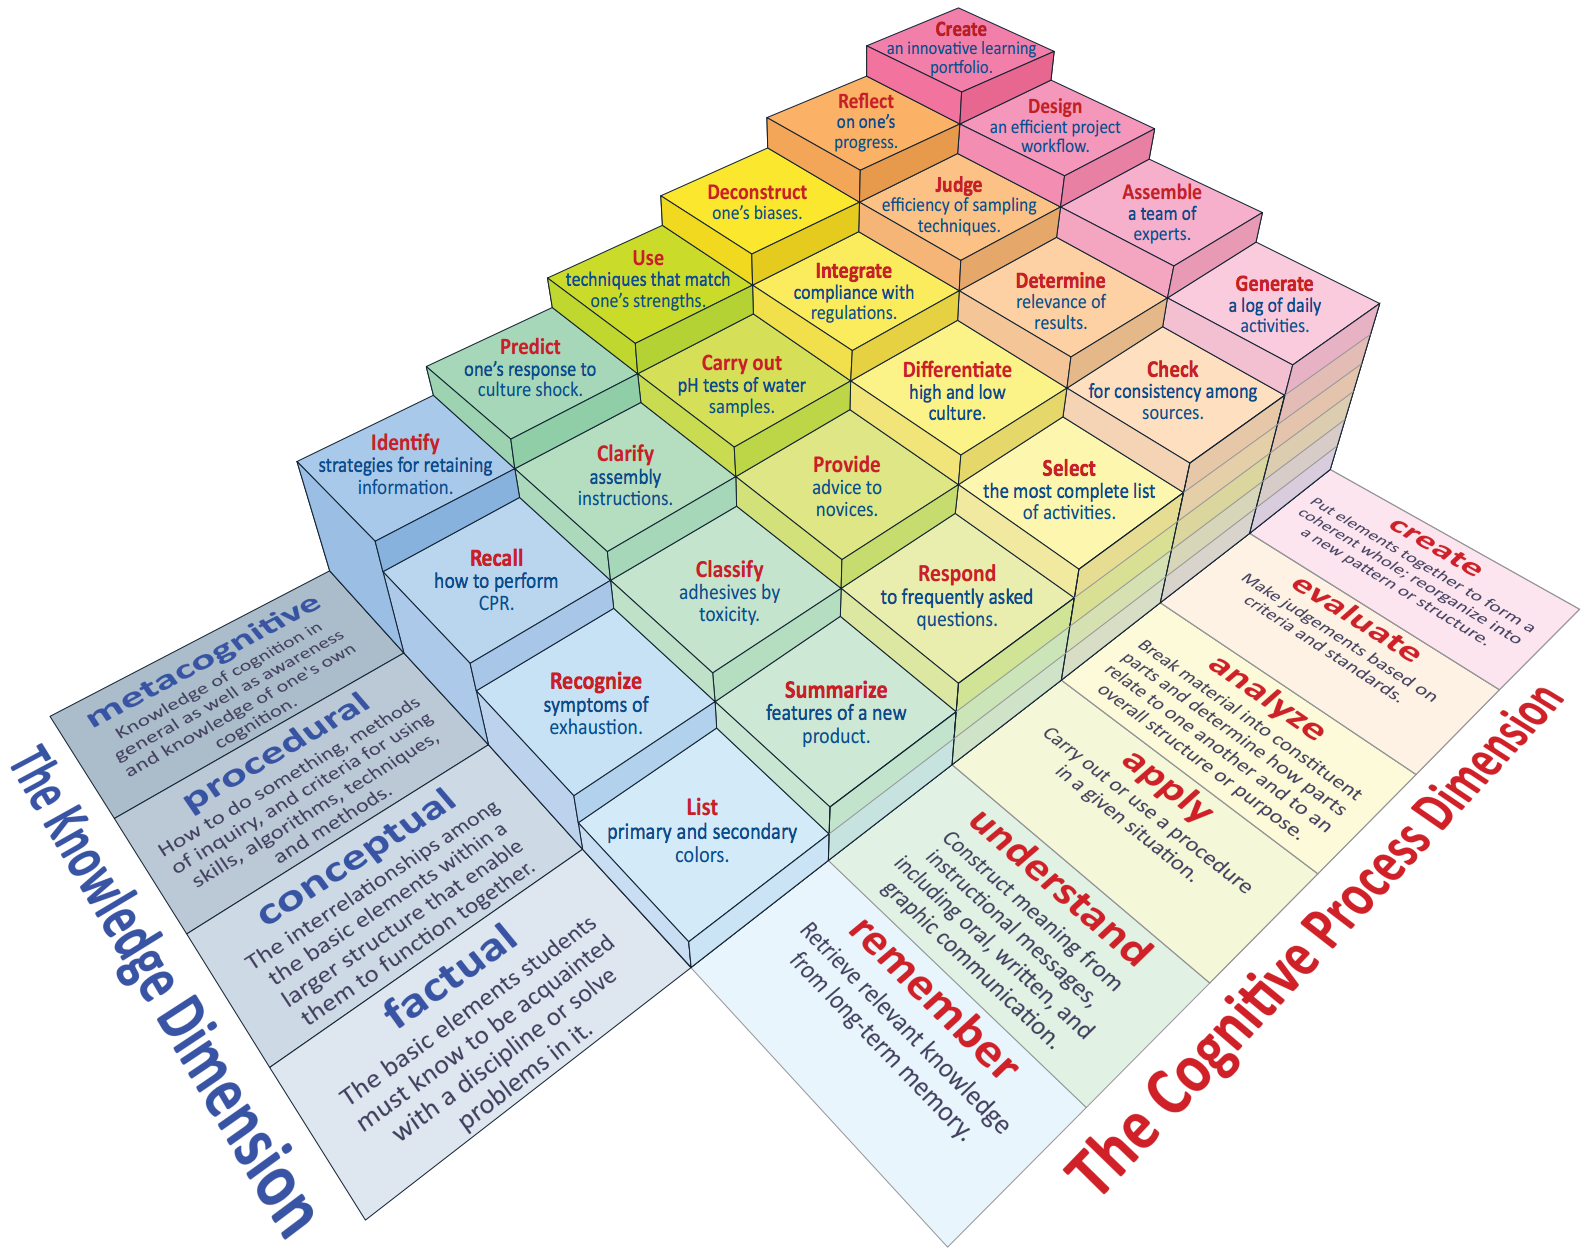
\includegraphics[width=1.0\textwidth]{RevisedBloom.png}
    \caption{Bloom's revised taxonomy visualised with examples of different learning objectives.}
    \label{fig:revised-bloom}
\end{figure}

  Learning activities often involve both lower order and higher order thinking skills as well as a mix of concrete and abstract knowledge.

  The taxonomy can provide usable insight into how to design, by the combination between lower or higher cognitive complexity, and concrete (factual or conceptual) or abstract knowledge (procedural or metacognitive). \cite{cheong}

  \subsubsection{Building skills: by Spaced practice, Deliberate practice and Perceptual exposure}

  Spaced practice deals with spreading out learning, with the purpose of not forgetting. E.g. Gates \cite{Gates} concludes that spaced learning versus massed learning did have a memory benefit in their study.

  Designing for this, could mean making the user apparent on the person's meta-cognitive ability (personal insight into what you'll remember), and meta-memory (when you need to repeat information in order not to forget).

  Moreover, dividing learning into 45-90-minute chunks, getting to 95\% reliable within three sessions, has been proven highly effective. This is called deliberate practice. Gates \cite{Gates} agrees, finding no evidence of consistent correlation between total duration and effects on learning outcomes in their study.

  Sierra presents a number of strategies, most notably research within deliberate practice \cite{yengin} \cite{sierra}. Deliberate practice has been proven to be an effective way to build skills. It has also been tested before for mobile learning environments. \cite{yengin}

  Sierra \cite{sierra} suggests skills to be divided into three buckets: can't do (but need to do), can do with effort, and mastered (reliable/automatic). The goal then is to move skills from can't do into mastered, in the best way possible. See figure \ref{fig:sierra-practice} from Sierra \cite{sierra}.

  \begin{figure}[h]
    \centering
    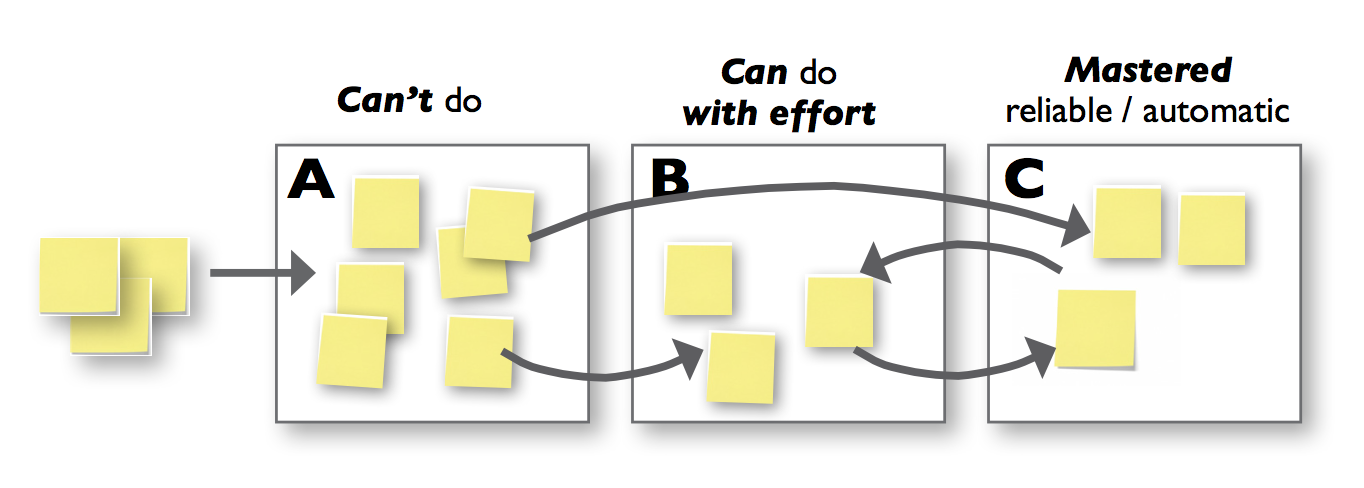
\includegraphics[width=0.8\textwidth]{SierraPractice.png}
    \caption{Moving skills from A (Can't do) to B (Can do with effort) into C (Mastered) can move different ways, depending on how effective the learning is. Deliberate practices focuses on A-B-C, while perceptual expose enables A to C. Reflection allows knowledge to go backwards, to get better at the skill than previously possible.}
    \label{fig:iterationprocess}
\end{figure}

  Desirable difficulties applies here, meaning that during deliberate practice, it may feel as if learning gets harder and harder, but in the long term the user is actually learning more. As a result, less people does true deliberate practice, but they do not get the same reward in return. This needs to be designed for, e.g. using social psychology.

  A way to build skills quickly, is to utilize that the brain is brilliant at pattern-matching, by the method "perceptual exposure". \cite{sierra}

  By exposing users to very high-quality samples during a very limited time, experts can learn intuitively.

  \subsubsection{Learning from Assessment}

  Knowing what learners know, and don't know, is crucial to effective learning, Luckin \cite{luckin} says.

  Assessment can partly help to design for flow, matching challenge and ability \cite{bruhlmann}, which is effective for intrinsic motivation (see next chapter).

  Moreover, it also has cognitive benefits. It can help to offer appropiate feedback, increase learners' awareness of their learning needs, and give accurate assessment and analysis, and allows learning to be tailored.

  By recognizing differences of students, in their ability to understand what they know and how they can progress, it is possible to ensure that everyone achieves their full potential.

  Effective assessment by a teacher or agent includes individual feedback (task-oriented and informal) and appropiate feed-forward advice.

  \subsubsection{Learning by Thinking: Reflection \& Retrieval Practice}

  When reflecting, the student develops neccessary skills and self-awareness to refine their own learning activities. This surely applies to the teacher as well, Luckin says. \cite{luckin}

  Stefano \cite{stefano} suggests that that reflection has been an overlooked area of research for a long time.

  They found that individuals who are given time to reflect on a task, outperforms students who are given the same amount of time to practice with the same task.

  His results suggests that reflection as an activity that can be more effective than additional learning.

  Similar to deliberate practice, it is a desirable difficulty. Individuals in the test themselves, had a tendancy to allocate time to practice on the task rather than reflecting on it.

  %\subsubsection{Retrieval practice}

  Bjork \cite{bjork} shows that retrieval from memory is more effective than people who repeat reading the same thing to remember.

  They also showed, that the more effective students, retrieves from memory.

  E.g. "What was in that article?", instead of immediately reading the article, is an example of memory retrieval that is extremely effective for learning, their research shows.

  One design method to encourage this, would be flip cards, where the question is on one side, the answer is on the other, versus giving the person a multiple-choice question.

%\subsubsection{Not forgetting}

%UCLA Bjork's Learning and Forgetting Lab researches how people forget, and how to design so that people do not forget.

%\include{theory/learning/pedagogical-development/social_psychology}



\subsection{Methods to Design for Motivation}

Social psychology can guide the design, when there is a wish to make people behave differently. A big research area is motivational psychology.

With a compelling context, the users are already motivated. Their motivation, is to become better.

Sierra \cite{sierra}, instead suggests the focus to be how to help users progress (see "Progress and payoffs"), and what pulls them off (see "Cognitive load theory").

\subsubsection{Cognitive load theory}

Sierra argues working on what stops people, matters more than working on what entices them. Thus, a focus needs to be identifying and removing blocks.

Sierra \cite{sierra} describes how humans have scarce cognitive resources, and how to design for these.

Cognitive load theory research is divided into three areas: intrinsic CBT, extrinsic CBT, and germane CBT. Below, to design for these are described.

Intrinsic CBT, needs to be dealt with if the effort is too high. Sierra \cite{sierra}describes two strategies. She first says that according to deliberate practice, if you can not get to 95\% reliability within three 45-90 minute sessions, split skills that can be done with effort into sub-skills. The purpose is to reduce time spent practising being mediocre.

Extrinsic CBT, the way presented to a learner, should be handled via designing to support cognitive resources, Sierra says \cite{sierra}.

Scaffolding is a technique to step by step remove the support wheels for the user, e.g. present information in different ways. Gates' \cite{gates} report shows that in their research, each category of scaffolding demonstrated significant effects on learning.

Also, reduce cognitive leaks by e.g. don't make them memorise, and make the thing you want the user to do, the most likely thing to do (affordances). Everything that takes willpower, reduces cognitive leaks.

Germane CBT, is the work put into creating a permanent store of knowledge. To support cognitive resources, escape the brain's spam filter by making the information essential. Either by designing for the compelling context, or desining for just-in-time learning versus just-in-case, Sierra says. \cite{sierra}

\subsubsection{Progress and payoffs}

Sierra aruges that to pull users forward, to stay motivated, progress and payoffs are essential. Both of these, are investigated in terms of motivational psychology.

The feeling of progress can be emphasised by a path with guidelines to help the user know where they are at each step, e.g. for a training.

The best payoff, is a intrinsically rewarding experiences, according to Sierra \cite{sierra}.

It is superb to gamification, says Sierra \cite{sierra}. This is in-line with self-determination theory, where e.g. Pink \cite{pink} says that the surprising truth about what motivates us is that drive is fostered by autonomy, mastery and purpose. The most efficient way is therefore to design for having intrinsically rewarding experiences.

Caring for the compelling context, why the user wants to learn the skill, are helpful strategies. Other strategies are flow, mentioned before, or to give high pay-off tips, helping the user progress in a fair way.

Gates \cite{sierra} says that simple gamification as well as more sophisticated game mechanics can prove effective. However, they add that it should be investigated if "simple gamification" (e.g. contingent point and badges connected to learning activities) more frequently focus on lower-order learning outcomes, compared to studies with more sophisticated game mechanics.


\section{Setting and research context}
Uganda (Kampala, Tororo) and Zambia (Kabwe).

\section{Subjects (Participants) \& Stakeholders}

Lorum ipsum.

\section{Study Design \& Data Collection}

\subsection{Interdisciplinary Design Process}

%\subsection{Digital Learning}

%\citep{edtech-clark}
%\citep{edtech-sjoden}
%\citep{edtech-dangelo}

\subsubsection{Mobile Learning}

\textbf{The use of deliberates practices on a mobile learning environment}

TODO, superbra artikel

\textbf{An experiment for improving students performance in secondary and tertiary education by means of m-learning auto-assessment}

Luis de-Marcos

% Proved successfull, everyone improved their knowledge. I can use a similar methology, and compare to the development context.

--

Huang et al. (Huang et al., 2008) indicated the common problems encountered in m-learning applications: (1) software integration, (2)
limitations of the web browser, (3) interface usability, (4) reduced size of the screen, and (5) limitation of the battery life. Such limitations are
of particular relevance when the application is intended to run on students’ personal phones; in this case, decisions need to be taken in an
attempt to alleviate the impact such issues may have. Of the problems listed above, item 2 can be mitigated by developing a mobile
application that does not run on the web browser. Items 3 and 4 can be alleviated by designing an interface that minimizes the amount of
information displayed and the input required from the user. This was the main reason for preferring multiple-choice questions to other
kinds of questions, since these questions can usually be stated in a few lines and require the selection of one or more choices. A few mobile
phone buttons can then be programmed to select/unselect each option. Moreover, various experimental studies (Chen, 2010; Ventouras,
Triantis, Tsiakas, \& Stergiopoulos, 2010) support the validity of this assessment method. Solving the problem represented by item 5 was
beyond the scope of this study; however, students were advised to charge their devices before taking the tests and teachers were advised to
design tests of no more than approximately 10 questions, in order to reduce connection times to a maximum of 20 min. Finally, item 1 was
especially difficult to tackle. When the technological framework was set up, our decision was to define the minimal software requirements
that handheld devices would have to meet in order to run the application.

% NTA Digital, Om Digitalt Lärande, Att lära med digitala verktyg
% http://ntadigital.se/teacher/tutorings/2

Interaction design talks about the creation of digital artefacts specifically. When it comes to the design process, it is influenced by related areas such as human-computer science, and more recently human-centered design.

However, various disciplines suggests different design processes. For example, agile development suggest how do develop software efficiently.

Whenever a project is multi-disciplinary, various design processes may need to be combined. Whenever this happens, design thinking becomes a skill essential to thoughtfully design the process.

Löwgren \cite{lowgren} writes about design thinking and useful techniques in general, from his interaction design perspective.

Service design thinking connects various fields of activity \cite{stickdorn}, and it's methodology relies on being close to the users.

While interaction design talks about the creation of digital artefacts specifically, service design talks about the creation of services.

As some digital artefacts are used within a service, or can be thought of as both a product and service simultaneously, the combination of the two are very useful.

Each discipline holds efficient methods and tools, that can be modified to suit the specific situation even better. From the field of graphic design, mental models are usable. From interaction design, desirability, utility, usability and pleasurability are useful principles. While not naturally a part of service design, these have been useful in service design projects previously. \cite{stickdorn}

In difficult situations, this places demands on the designer. This is where design thinking becomes relevant.

Here, relevant methods and tools are briefly described, and what it means to be a good designer.

\subsubsection{A good designer}

The result of a method can not be better than the people engaging in carrying out the process \cite{lowgren}.

With its user-centered and T-shaped focus \cite{stickdorn}, service design can be said to equip the designer with tools both for reasoning and design ethnography.

This is neccesary, as a good designer can deal with the complexities of design: a satisfactory (and surprising) solution or design can be achieved while working in a highly restricted situation.

\subsubsection{How to deal with relationships and roles}
According to Löwgren, "real" design is about finding ways to design a project within the existing preconditions and limitations \cite{lowgren}.

While a researcher is interested in reality, a designer is interested in what reality could become. \cite{lowgren} Being thoughtful means conceptual clarity from the designer, caring for the vision, and being equipped with appropriate tools of reasoning.

There are three roles as interaction designer in particular can take: the computer expert, the socio-technical expert, and the political agent. The trend is increasingly towards socio-technical experts \cite{lowgren}, the middle ground.

This seems to be a perfect fit with service design, where interaction design is both technical skills and design, and service design can be both design and ethnography. Even more importantly, service design suggests making the whole process co-creative, involving all stakeholders. \cite{stickdorn}

\subsubsection{Thinking of a product as a service}

Service design thinking is described as a process of designing, rather than to its outcome.

A service's intent is to meet customer needs. If it does, it will be used frequently, and recommended. \cite{stickdorn}

As this is often not the case, service design can be applicable to fields including social design, product design, graphic design and interaction design.

The result can be a product service hybrid. When designed and considered well, service design shapes the value proposition and desirability of the product for the better.


\subsubsection{Service design methodology}

Below, brief descriptions of the five principles of service design is described, together with how the work is divided into iterations, and examples of tools that can be applied.

\subsubsection{Service design principles}
Stickdorn \cite{stickdorn} describes five principles that constitute service design thinking, and how to follow these.

The book describes how to follow these principles, by making the process user-centered (e.g. via design ethnography), co-creative (involve all stakeholders) and holistic (keep the big picture). Sequencing (visualize the service, and make iterations) evidencing (make the service tangible) are the two last important principles.

\subsubsection{1. Sequencing: The iterative process}
While literature and practice refer to various frameworks, with different number of steps, every service design project includes: exploration, creation, reflection and implementation \cite{stickdorn}.

Nissar \cite{expedition-mondial} suggests a model where one iteration consists of insights, ideation, trigger material, and interactions. See figure \ref{fig:iteration}.

\begin{figure}[h]
    \centering
    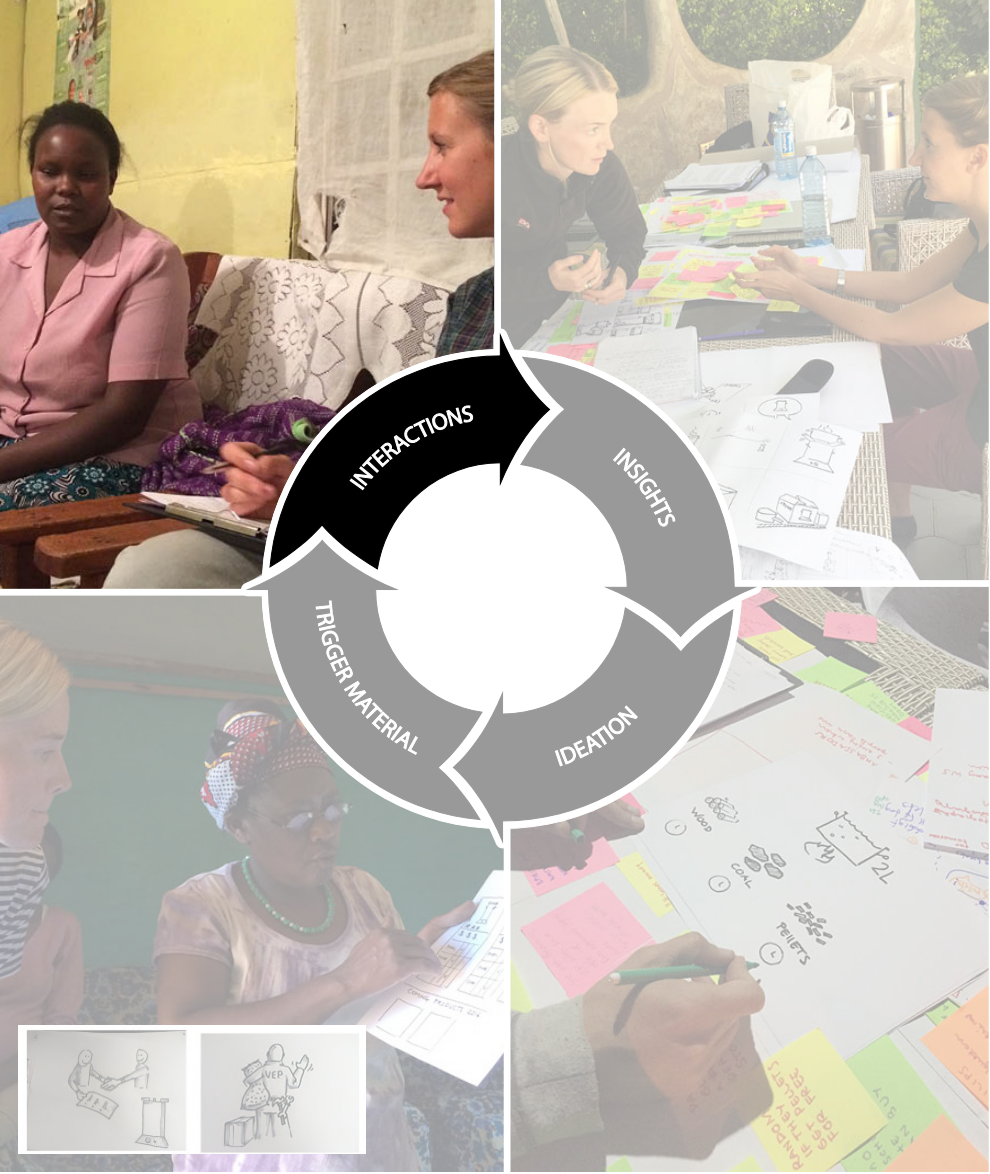
\includegraphics[width=0.7\textwidth]{Iteration.png}
    \caption{In Nissar's model, a iteration consists of Interactions, Insights, Ideation and Trigger material.}
    \label{fig:iteration}
\end{figure}

\begin{enumerate}
\item Interactions, where you are listening, the \textit{Explorative phase}.
\item Insights, which is where you use the Interactions in order to try to understand, the \textit{Understanding phase}. % better word+
\item Ideation, where you find possible ideas and when creation of new version of the app is done, the \textit{Design phase}.
\item Trigger material, where material is developed to test the outcome of our evaluation in the next round, the \textit{Trigger development}.
\end{enumerate}

The iterations should come closer and closer to a desired outcome. It is not always obvious what this outcome is. For each iteration, the process takes the project closer, from Why? to What? to How?, often with overlaps \cite{expedition-mondial}. See figure \ref{fig:iterationprocess}.

%\begin{wrapfigure}{r}{0.25\textwidth} %this figure will be at the right
%    \centering
%    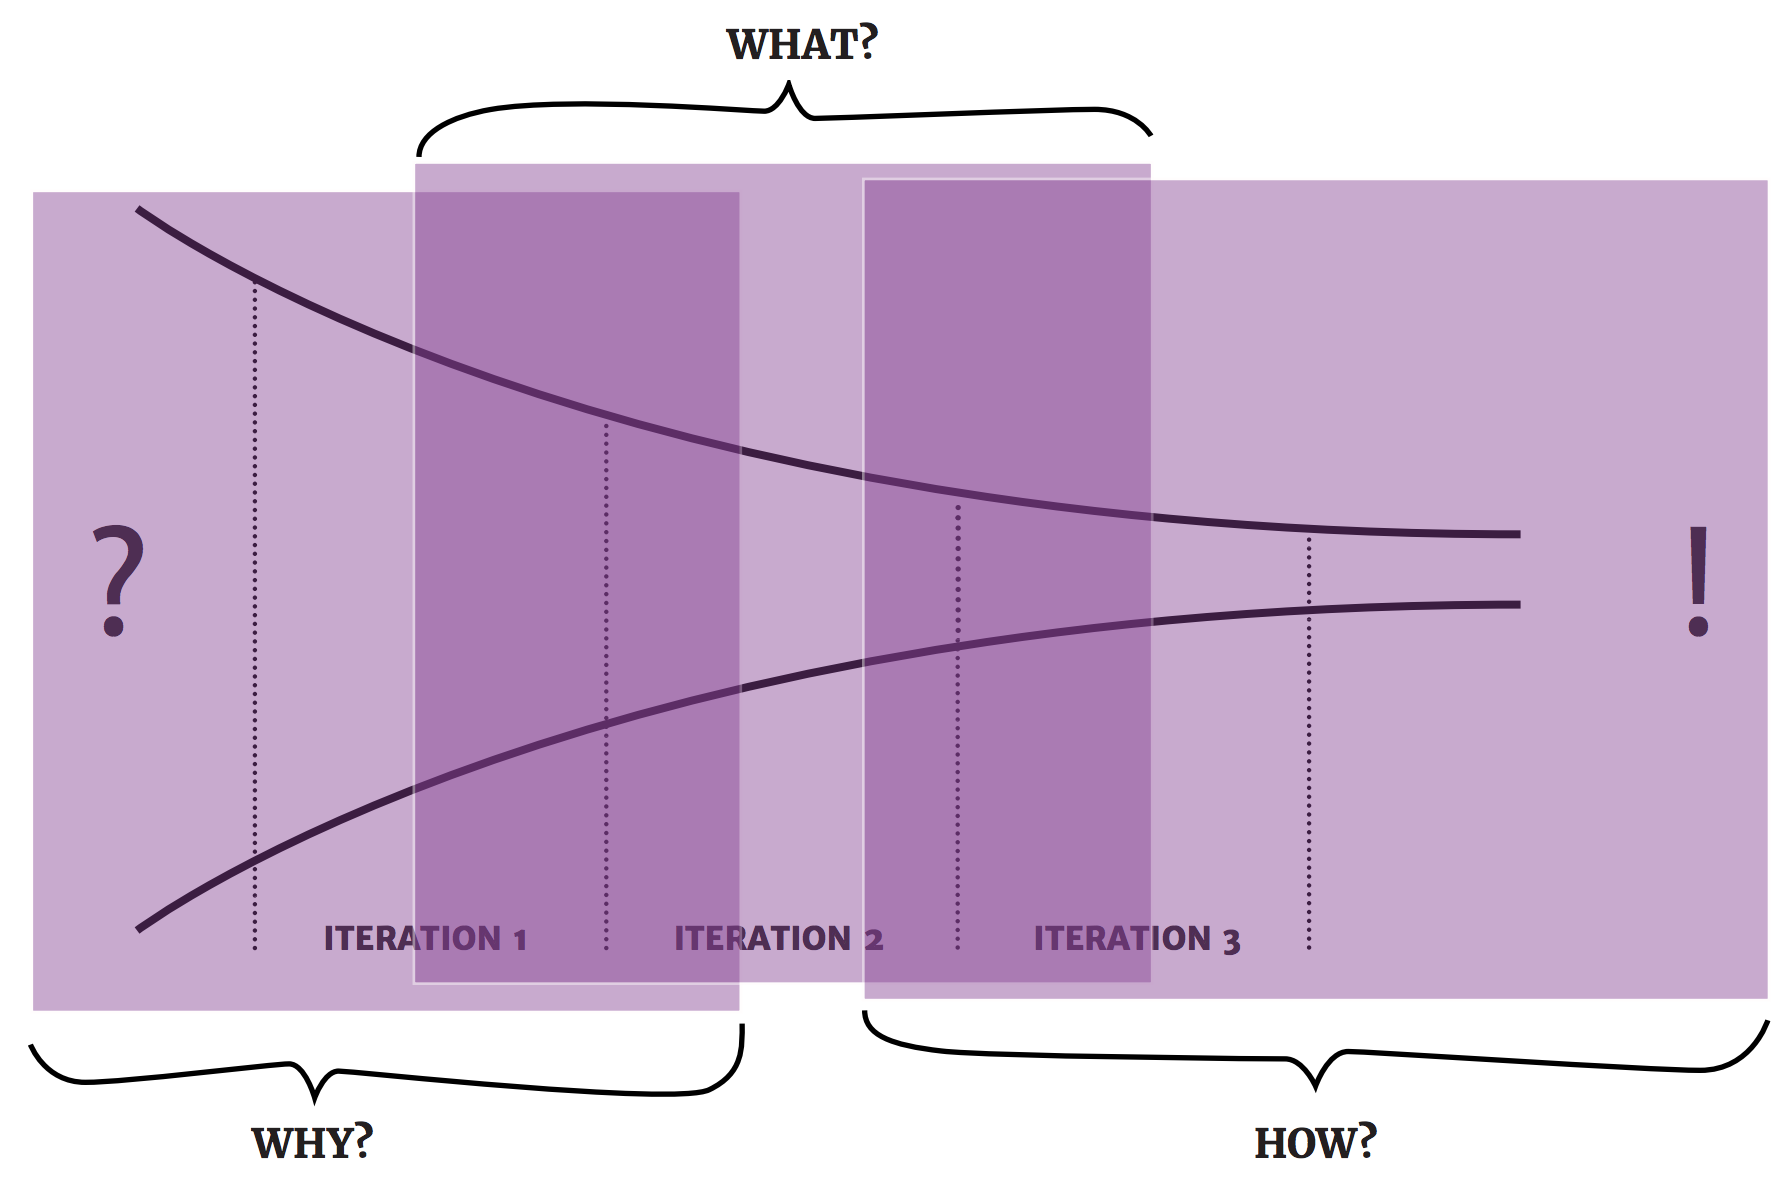
\includegraphics[width=0.25\textwidth]{IterationProcess.png}
%    \caption{Iteration process}
%    \label{fig:iterationprocess}
%\end{wrapfigure}

\begin{figure}[h]
    \centering
    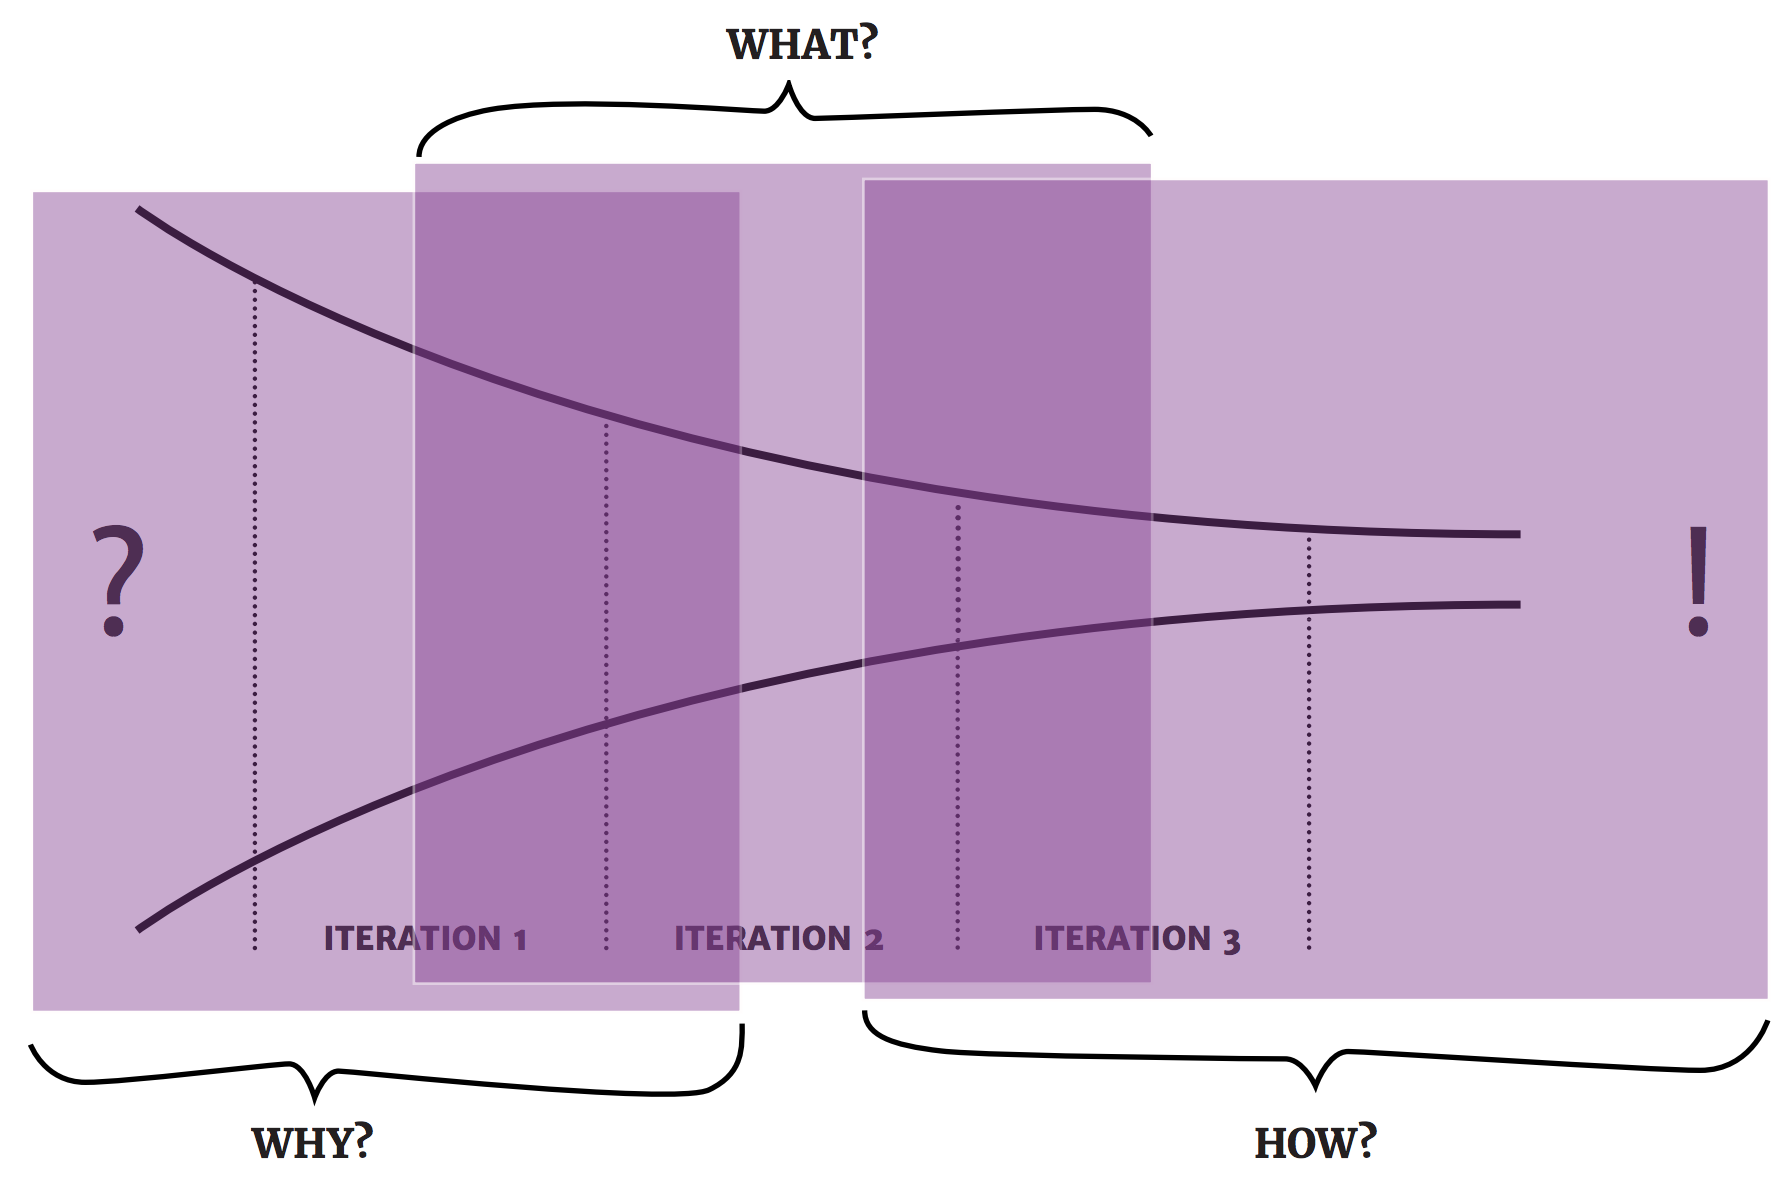
\includegraphics[width=0.8\textwidth]{IterationProcess.png}
    \caption{The iteration process consists of a number of iterations with different focus, starting with broad strokes, and narrowing down into a concrete product. Between iterations, the overlap between "Why?" and "How?", "How?" and "What?", signals that there is a learning process which means conclusions may need to be quickly questioned as new insights emerge. This is especially important in projects where you work with an unfamiliar target group and there are several uncertainties and constraints.}
    \label{fig:iterationprocess}
\end{figure}

\subsubsection{Service design tools}

There are a number of popular service design tools that follows the five principles, e.g. how to make it user-centered.

Explorative tools are e.g. Shadowing, Customer Journey Map, Contextual Interviews, The 5 Why's (same as "Why-why-why" within interaction design \cite{thoughtful}), Cultural Probes, Mobile Ethnography and Personas.

Tools to create and reflect can be done via a certain work methodology, e.g. agile development, and structuring and inspiring brainstorms, e.g. via "What if...?" and Co-Creation, inviting stakeholders in the creation process.

%\subsubsection{Relevancy within Social Innovation}
%\citep{socialinnovation-ehn}

%\subsubsection{Service Design Thinking}

%\subsubsection{Methodology}

\textbf{The iteration process}

The time in Uganda is divided into three iterations. For each iteration, the result becomes more and more clear. In iteration 1, there is a very broad scope, without digital focus whatsoever, where iteration 2 and 3 gradually introduces the digital solution. See figure \ref{fig:iterationprocess}.

%\begin{wrapfigure}{r}{0.25\textwidth} %this figure will be at the right
%    \centering
%    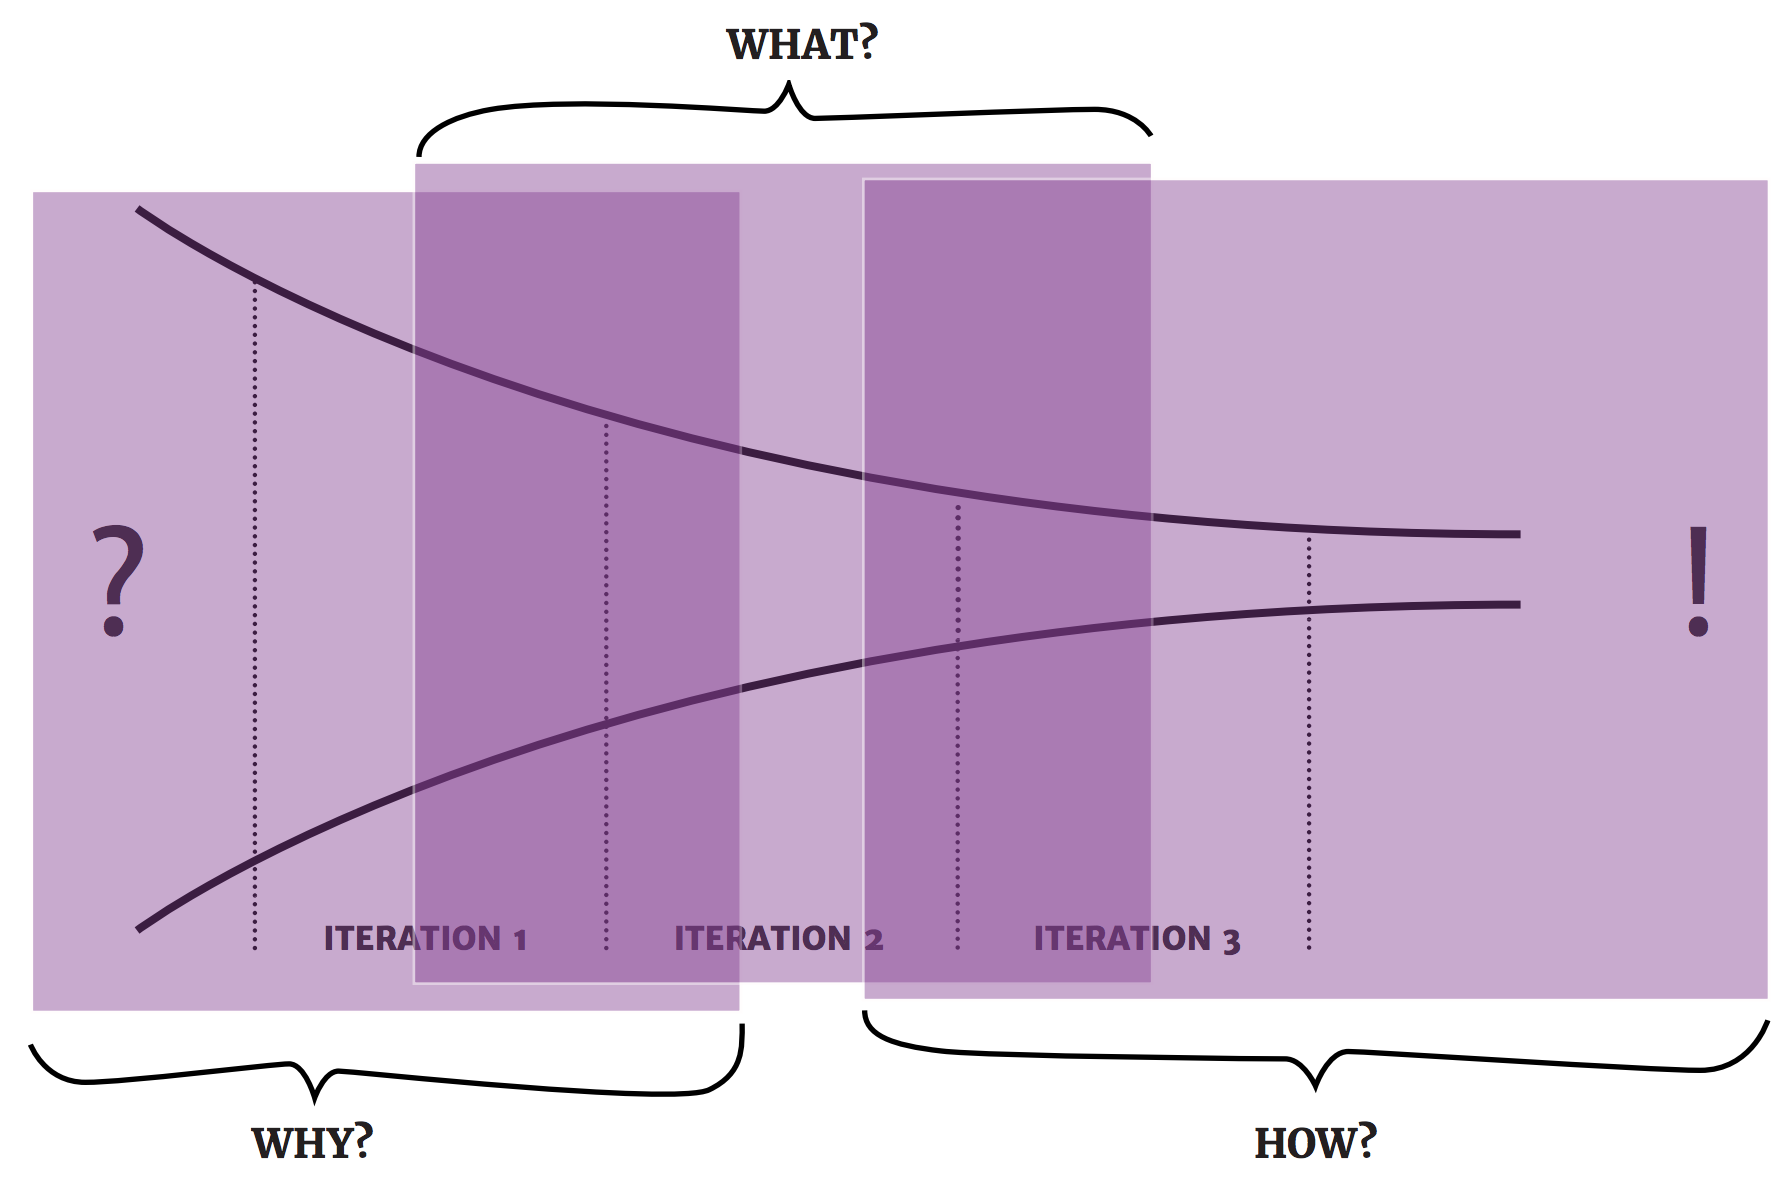
\includegraphics[width=0.25\textwidth]{IterationProcess.png}
%    \caption{Iteration process}
%    \label{fig:iterationprocess}
%\end{wrapfigure}

\begin{figure}[h]
    \centering
    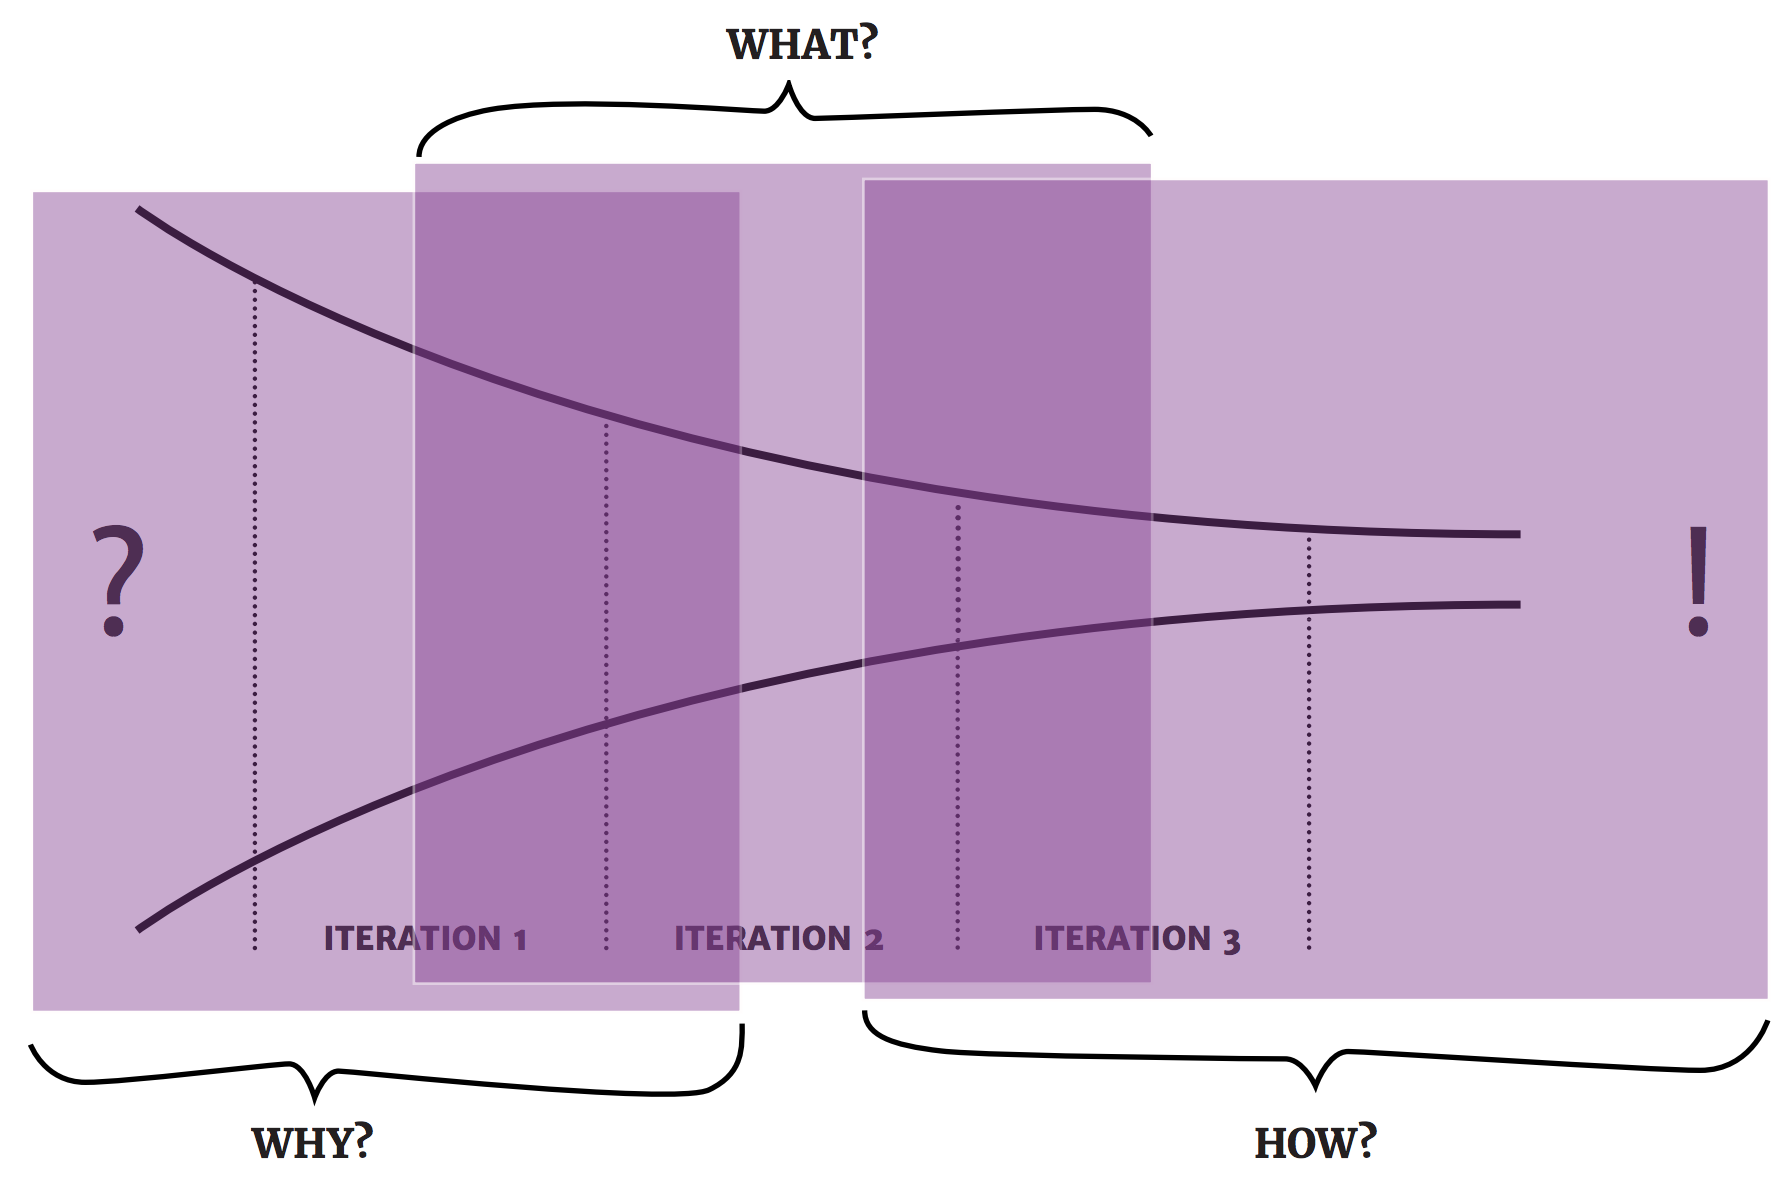
\includegraphics[width=0.8\textwidth]{IterationProcess.png}
    \caption{The iteration process consists of a number of iterations with different focus, starting with broad strokes, and narrowing down into a concrete product. Between iterations, the overlap between "Why?" and "How?", "How?" and "What?", signals that there is a learning process which means conclusions may need to be quickly questioned as new insights emerge. This is especially important in projects where you work with an unfamiliar target group and there are several uncertainties and constraints.}
    \label{fig:iterationprocess}
\end{figure}

\textbf{One iteration} \\
In the way of reasoning around development and design for learning, the steps for each iteration, see figure \ref{fig:iteration}, might be translated into:

\begin{enumerate}
\item Interactions, where you are listening, the \textit{Explorative phase}. 
\item Insights, which is where you use the Interactions in order to try to understand, the \textit{Understanding phase}. % better word+
\item Ideation, where you find possible ideas and when creation of new version of the app is done, the \textit{Design phase}.
\item Trigger material, where material is developed to test the outcome of our evaluation in the next round, the \textit{Trigger development}.
\end{enumerate}

%\subsection{Service Design}
%\citep{servicedesign-ruth},
%\citep{servicedesign-balis},
%\citep{servicedesign-ruth}
%\citep{servicedesign-ideo}
%\citep{servicedesign-stickdorn}

\textbf{The purpose}
Applying service design serves two purposes:

Going from being a computer expert into a socio-technical expert,
In particular, the approach of service design refers to the process of designing rather than to its outcome. (This is Service Design Thinking, 2010, s. 7). ("The outcome of a service design process can have various forms: rather abstract organisational structures, operation processes, service experiences and even concrete physical objects.")

\textbf{The need for service design (in my project)}

\textbf{About service design}
Since service design is a still young and emerging approach, service design education is even younger and just developing. (TISD, 2010)

Without a doubt, you cannot learn what service design is and how to do it just from a textbook. You need to try, fail, learn from your mistakes, improve, try again and thus educate yourself.

Service design education is therefore rather a kind of briefing and tutoring process. Besides explaining the big picture, it is all about giving hints, proposing methods and tools, and showing how to use them while working on a project.

Service design as a practice generally results in the design of systems and processes aimed at providing a holistic service to the user.

Service Design helps to innovate (create new) or improve (existing) services to make them more useful, usable, desirable for clients and efficient as well as effective for organisations.

Service design is all about making the service you deliver useful, usable, efficient, effective and desirable. (UK Design Council, 2010)

(kan lägga till bild)

What distinguishes service design is:

5 principles of service design thinking
Marc Stickdorn
1. User-centred
Services should be experienced through the customer’s eyes. 2. Co-creative
All stakeholders should be included in the service design process.
3. Sequencing
The service should be visualised as a sequence of interrelated actions.
4. Evidencing
Intangible services should be visualised in terms of physical artefacts.
5. Holistic
The entire environment of a service should be considered.

According to TISDT (2010), there is the Customer, Service Provider, Stakeholder, and the Service Designer.

There is then the Touchpoint (every contact point between a customer and the service provider), Service Evidence (a tangible artefact related to a service process), and Service Period (pre-service / service /post-service --current period of a service).

% Här är jag nu i exjobbsrapporten - HÄR

\textbf{How to make it user-centered: TISDT (2010) and Contextual Design (X)}

Agree on a common language!

services are created through interaction between a service provider and a customer. The inherent intention of a service is to meet the customer’s needs and, as a result, be used frequently and recommended heartily. This is often not the case.

Though statistical customer descriptions are important, a true understanding of habits, culture, social context and motivation of users is crucial. We need to put the customer at the centre of the service design process. This requires a genuine understanding of the customer beyond mere statistical descriptions and empirical analyses of their needs. Gaining authentic customer insights includes the application of methods and tools that enable the service designer to slip into the customer’s shoes and understand their individual service experience and its wider context. We are all customers – though with different needs and mindsets. The understanding and disclosure of these disparate mindsets is where service design thinking begins.

we all have individual backgrounds and experiences. The ability to make use of this knowledge during the development of services is crucial for its later success. A user-centred approach offers a common language we can all speak; the service user’s language.

\textbf{Making it co-creative}

This is co-creative.
A broad understanding in various disciplines and a deep knowledge in a specific field is crucial for co-creative work in interdisciplinary teams.


Putting the customer at the centre of a service design process involves facing the reality that potentially there is more than just one customer group, and each group possesses different needs and expectations.
Furthermore, providing services also demands consideration of the various stakeholders,

How can we integrate the stakeholders of a service into the process of designing it?

There are a variety of methods and tools for gaining genuine insights from different user perspectives in the creation of services and for the development, prototyping and testing of these service concepts. This is co-creation, and facilitating this in groups representative of your stakeholders is a vital aspect of design thinking and a fundamental part of service design.

co-creation during the design process facilitates a smooth interaction between the stakeholders during the actual service provision – essential for both sustainable customer and employee satisfaction. Through co-creation customers get the chance to add value to a service in partnership with the service provider early in the development of the service. The more a customer gets involved in the service provision, the more likely this service is of evoking co-ownership which in turn will result in increased customer loyalty and long-term engagement.

\textbf{Making it into sequences} %Chapter: It is sequencing

This is Sequencing.
The series of interactions outline a so called customer journey through the offerings of the respective service.

Imagine a very simple example of a service such as going to a hairdresser. Now try to visualize this service process as
stage play or movie. This movie would consist of a series of static pictures, which would be combined to create a moving sequence. Service design thinking uses this analogy to deconstruct service processes into single touchpoints and interactions. These, when combined, create service moments. Touchpoint interactions take place human-human, human-machine and even machine-machine, but also occur indirectly via third parties, such as reviews from other customers or via print or online media.

Every service process follows a three-step transition of pre-service period (getting in touch with a service), the actual service period (when the customers actually experience a service) and the subsequent post-service period.

Like a stage play, a service moment not only consists of what is happening front of stage, it also includes multiple backstage processes such as cleaning of the shop
33
floor to prepare the front of stage for action. To achieve an excellent theatrical performance, actors have of course to run through many rehearsals; services are no different. We need to prototype services and iteratively test their impact on customers.

\textbf{It is evidencing}

% OBS: korta ner! Ta inte mer så mycket av detta i teorin, för det blir jobbigt att följa upp på.

Make the intangible tangible!

Services often take place unnoticed in the background, like the housekeeping service in a hotel. In fact, services like these are intentionally designed to be inconspicuous. However, if paying a bill is the first moment customers become aware of such backstage service processes, their inconspicuousness might create a disparity in customer expectation and potentially result in their disaffection with the service.

Physical evidence or artefacts such as souvenirs or small bottles of shampoo from your hairdresser can trigger the memory of positive service moments and thus, through emotional association, continue to enhance customers’ perceptions of the service they have received.

Service evidence can thus prolong service experiences beyond the mere service period far into the post-service period. Utilising this effectively has the potential to increase customer loyalty and for customers to recommend the service to others. %Här finns en uppenbart grym koppling till Badass: Making Users Awesome!

In addition, evidence can explain certain aspects of a service touchpoint or process, a sign next to an electric hand dryer pointing out that the proprietor knows that customers would prefer to use real towels but that costs or the environmental impact do not allow this can generate appreciation and empathic engagement.

Evidencing can occur in a variety of forms: bills, mail, emails, brochures, signs, souvenirs or other pro-ducts. These add a tangible component to what would otherwise have been an intangible experience.

Service evidence needs to be designed according to the service’s inherent story and its touchpoint sequence. If a service process is like a movie, a better understanding of the work behind the scenes (i.e. the backstage processes of services) can result in an increased customer appreciation of the service experience.

\textbf{It is holistic}

Keep the big picture!

Which aspects need to be considered when designing services?

the intention should always be to see the wider context in which a service process takes place.

At the level of individual touchpoints and service moments, the focus should be on the environment where the service takes place. The conscious awareness of what customers might otherwise perceive subconsciously with their senses can have a profound impact on the experience of the service itself.

% Detta kanske jag inte tar med?
At the level of the service sequence, there should be a focus on alternative customer journeys. There are always a number of alternative touchpoints and approaches, which need to be taken into account. Sequences change and need to be repeatedly reappraised from various perspectives to ensure a great customer experience. Hence, it is important to map the mood and feelings of all stakeholders throughout the service journey.

To summarise, service design thinking supports the co-operation of different disciplines towards the goal of corporate success through enhanced customer experiences, employee satisfaction, and integration of sophisticated technological processes in pursuing corporate objectives.

\subsubsection{Who are these Service Designers?}

Service design thinking as an interdisciplinary approach includes and connects various fields of activity.

\textbf{Product Design: developing products with service applications (TISD, s. 50)}
This chapter looks at the influences of service production upon product design and considers the implications of the evolution of product designers from designing just products to designing services too.

Design is arguably now focused on the interaction between people and technology, and products serve as platforms for experiences, functionality and service offerings (Buchanan, 2001).

Designers study users and their usage of artefacts to develop better products and generate knowledge that can be embedded into artefacts.

Users generate knowledge through interpretation of this embedded knowledge in artefacts. They need to be able to understand the value, meaning, and the ways to use the artefact in different situations of their daily lives.

\subsubsection{This is co-creative}

The concept of activity refers to participants’ interactivity, initiative and style of collaboration and contribution in design events. User roles may vary from proactive participation where users contribute to solving and framing design challenges to passive roles where designers instead interpret user data without any direct engagement with the user community (Keinonen, 2009).

\textbf{Iterative design development} helps to solve problems found in user testing. There must be a cycle of design, testing and measurement, then redesign, repeated as often as necessary. This is a way to incorporate results of behavioural testing into the next version of the system. Making a system user friendly and easy to operate is the goal of this approach (Gould and Lewis, 1985). Iterative design is a design methodology based on a cyclical process of prototyping, testing, analysing, and refining a work in progress.

Both conceptual and iterative design approaches are important phases in the service design process. The challenge is to design user-orientated hybrids that incorporate both the customer facing products and that help articulate the service they assist in offering.

\textbf{Product-service hybrids}

Koivisto (2007) defines hybrid products as products where the service has been designed as an inseparable part of the product. % A good example of this is Apple’s iPod and iTunes product package (Apple, 2010). Developing such a hybrid product means that both the product concept and a service system are developed in tandem.

A successful service design project requires integrating stakeholders as earlier as possible in the project development process. Opportunities to iterate the product development process together with the stakeholders involved in the project should be created as soon as possible. This will in all likelihood result in an increase in proactive solutions. Management buy-in needs to be secured to support the process. There has to be constant communication, continuous sales work and partnership with the designers.

\textbf{Creating value propositions with users}

Mark Jones, Lead of Service Innovation at IDEO, says that from his perspective the design process begins with understanding the product’s context of use, and observation of users’ experiences by moving into the field to observe users and how they interact with the product. In a typical development project pre-research, work is done before one or two workshops with the stakeholders. Subsequently, the development case needs up to six or seven iterations and mock-ups as part of the iterative product development process.

Typically, a design team would consist of an engineer and designer. When you start designing actions, systems or product service systems, this range of expertise needs to be expanded through the involvement of a human factors expert. Design’s role is to illustrate and represent the complexity of the system to make it more understandable as well as represent the added value that the product brings to the company. Participatory design methods are used in the development work and this involves relating extensively with clients. How the methods are chosen depends on the business case.

% Detta går att diskutera under Future work, om att Plan vill använda verktyget till fler utbildningar, eller att YoungDrive vill bli ett socialt digitalt företag
When the product service systems or service-product hybrids are developed it’s not only about what kind of services are co-created with users but also about what the service’s role is within the organisation’s business model. When designed and considered well, the product service systems and service-product hybrids detailed here can make key contributions to the overall value proposition and desirability of the products offered by an organisation.

\subsubsection{Graphic Design: providing visual explanation}

Mental models help an individual’s orientation in the world; they are the abstract and reductive mental representation of the complexity all of us face in everyday life – the schemas by which all of us understand the world around ourselves.

%Koppla såklart till deras digitala kunnande
If, however, a user is confronted with a situation they have never previously experienced, they cannot fall back on an existing model.

The metaphor of the online shopping cart for example, promotes the development of a new mental model, through reference to an analogous experience. % The individual can draw upon known mechanisms and functionalities associated with, in this case, shopping carts to understand a novel and largely intangible online system of payment. Even though online shopping is phenomenologically different from previous experiences the user might have of “offline” shopping.

It is the graphic designer’s task to trigger an individual’s apriori mental models, or at least to positively influence the accrual of such cognitive representations of meaning.

This chapter explains what graphic design is capable of and what role it can play within service design – from the perspective of a graphic designer.

Two tasks: information and branding

% D.v.s., viktigt accosiera med YoungDrive, som de litar mycket på
Branding refers to helping an offering establish a visual identity and familiarity in the eyes of customers. Thus graphic design taps into and adopts a number of patterns of which the customer already has a mental model: use of the colour green in packaging can, for example, suggest an association with the user’s ideas of freshness, organic products or, more recently, environmental friendliness.

Information design, on the other hand, pertains to the task of making complex and abstract content accessible in a simpler way. Through logical composition, visual hierarchy and the use of visual metaphors, viewers are supported in their absorption and comprehension of information.

Branding supports the customer to emotionally approximate himself with the theme or emotional context of the experience.

Within this setting, information design leads to a satisfactory and positively associated user experience.

 It may be forgivable for a customer that their bank’s corporate identity does not really inspire confidence, but they become upset when they cannot see their balance because the pixelated letters on a screen are too small to read.

Visual presentation plays an important role in three ways. It pre-empts the actual service process, it controls customer expectation, and it can promote trust during interaction. The so-called look and feel can evoke a positive prevailing mood, or even makes the service usable in the first place through visual aides. Lastly, the visual appearance acts as an anchor that links the user to the positive experience. Visual control is henceforth a key competence in the conception of design propositions.

\textbf{Visual control}

For graphic designers it does not matter if they are working on a product or a service offering. Whether they have to create a print product, an interface or a three-dimensional presentation, it is imperative for the graphic designer to know what they want to offer the customer on a visual level, in order to adequately convey the thoughts and concepts standing behind the design proposition.

%It is nonetheless important to understand that the role of a graphic designer does not lie in sticking a previously developed logo on each and every surface. The complete visual appearance consists of far more factors than just such signage. The use of colours, text, photographs, the chosen medium, the type of production – there are countless ways to keep an image consistent and also countless ways to dilute it. As many parameters decide what is told by whom, as how it is told.

%The orchestration of these factors requires
designers to be open to current trends and familiar with previous trends to best enable them to understand the world of their target audience.

Branding and information design complement each other in a symbiotic way. Function and emotion combined define the concrete parameters like typography, colours, form and composition.

\subsubsection{Interaction Design: services as a series of interactions}

Services are a series of interactions between customers and the service system through many different touchpoints during the customer journey.

To value your customer, you need to spend some time understanding the interactions they have with your service, and that means two things. Firstly, viewing your service through the customers’ eyes, and secondly, designing in such a way that customers receive consistent experiences over time which they consider valuable. It’s strange, but repeatedly we see companies ignoring both of these aspects, with the consequence that customers feel ignored and value is lost.

digital interaction is an area that is becoming more and more central for service delivery.

\textbf{Desirability is king in the land of interface design}
% Desirability in a service fires desire in the customer. Desirable interactions are something you tell others about and which give trust with, and loyalty to, the service. Finally, and this is becoming more and more important, desirability has a strong emotional dimension, often giving a pleasurable experience from the interaction.

it’s not an easy thing to do, mostly because desirability requires collaboration across traditional silos in a service organisation.

\textbf{Utility - it just has to work at a functional level}

scoring highly in terms of utility demands that you really understand your customers and their needs, together with an understanding of the functional benefits of your design offering.

To get a high score on the utility level you need to offer people what they need but no more and this is not always an easy thing to pull off. There is a big tendency for feature creep in interactive services – hey let’s add that feature, it doesn’t cost extra!

This leads to a service that has strayed from the core offering and which customers find vague or fuzzy. Utility is about what your service does.

\textbf{Usability - Keep it simple, stupid (KISS)}
While utility is about what, usability is about how. Usability is all about how easy it is to get to the offering (utility value) when using the service.

It’s all about ease of use, which often relates to how quickly and smoothly a customer can move through the service journey, and the risk they run of misunderstanding something and making errors (and error recovery of course). Its key metrics are time, errors and flow.


Usability relates strongly to how the interaction is strung together, often in terms of the design of the dialogue between the (online) service and the customer. Within interaction design, this is often termed the interaction architecture, and describes the functional divisions between the different parts of a website, and upon the functional layout of a page. A website needs to be structured according to the customers’ expectations of structure. This is described as the customers’ mental model, and ideally, your website structure should mirror the customers’ mental model.

\textit{A good means of finding the customers’ mental model when designing a service is to ask customers to structure the site for you, and there are several methods available to help them do this in a structured way.}

% Väldigt bra innehåll, som hjälper mig!
There are three keys to unlock the door to usability: \textbf{frequency, sequence and importance}. Frequency says that things the customers do most frequently (e.g. next, back, search etc) should have a prominent position in the sequence. Sequence says that activities that occur in sequence should be presented in sequence (i.e. you pay at the end of a transaction, not in the middle). Importance means that important pieces of information need to be given clearly and at the right time (e.g. if you only ship within the EU, then a customer trying to buy from India needs to know this early on – not at the end of a six-page check-out dialogue). Understanding the customers’ mental model and applying the frequency, sequence and importance rule will crack most of your usability needs. But, beware, like all rules, you cannot follow them blindly, and there are always tradeoffs that have to be made between these elements.

\textbf{Pleasureability - the pleasure principle}
We like things that make us feel good. In fact, we use a lot of time, effort and money on pleasurable things. Why is it, then, that when it comes to digital interactions, most of it is designed to be neutral at best?

It’s as if we have all been brainwashed to expect utilitarianism in everything digital. Luckily, we are entering into the experience economy, in which, finally, pleasurable experiences are recognised as central in today’s markets.

Pleasurability is about how the whole solution makes you feel.


It relates to a sum of details within your service, and often relates this to culture from the world outside. Pleasurability relates to the way the interaction is designed. The way it looks, the way things move, the feedback it gives you. It relates to style, but it also relates to much greater things. It relates to your brand and to what people expect from you. Pleasurability is not something for everyone. Ryanair, for example, is fo-cussed upon the utilitarian value and explicitly distances itself from highbrow style in their interaction design, with great success. It focuses upon utility and usability as part of its utilitarian approach, and this links to its no-frills offering very well.

A high level of desirability requires strong internal alignment, a strong brand and knowledge of managing design. However, it is a very strong differentiator and gives a mind share amongst customers.

%Limitations: don't to this, it's too hard, and takes too long time
\textbf{Desirability – moving from good to great}
If you put some effort into your interaction design you will be able to make a perfectly good solution, but if you are searching for true desirability you need to work hard. The benefits can make it worth it, but you have to be very confident of your offering, your position, and have a crystal-clear brand to be able to move up the desirability scale.

\textbf{Conclusion}
To conclude then, it’s time for you to think about the mix of utility, usability and pleasurability that fits your service. The answer to this lies in understanding your customers, your offering and your brand strategy and in finding an alignment between the interactions you design into your service and what your company is all about.

\subsubsection{Social design: delivering positive social impact}

% Det här är bara en sidonot, men om en designstudent skulle stå i sitt bås och faktiskt *designa* under tiden, skulle det nog få väldigt mycket uppmärksamhet! Som en pop-up store.
% From this perspective, there is much to query and explore in the broader role of design disciplines and how they are positioned alongside other disciplines. Designers possess more than simply an ability to style products; they are practitioners of an applied process of creative skills: identifying problems, researching, analysing, evaluating, synthesising and then conceptualising, testing and communicating solutions. Design, whatever the discipline, is not only about an end product, but rather a systematic process of identifying problems, then researching, creating, testing and implementing solutions.

One can look to the design profession for inspirations on style, but further investigation will show that design offers more than solely the creation and promotion of consumer goods. It is also possible to observe that designers have, through their broad and adaptable skill set, a service to offer to all areas of society. Such broader applications of design have variously been termed \textbf{“innovation”} %Snygg brygga till innovation!
and “design thinking”, two terms that have seen David Kelley’s IDEO and D-School gain kudos in the pages of Business Week.

Employing the design process to tackle a social issue or with an intent to improve human lives is known as social design.

Methodologies of co-design, social innovation and service design have dramatically broadened the application of “design thinking”, giving impetus and stability to a social design movement. One could argue that through these new methodologies, designers are better communicating the value of their creativity.

Recognising the growth of a potential new design movement, many designers have begun forging multidisciplinary networks with the aims of social improvement through design.

\subsubsection{Technology in service design}
At McDonald’s, technology was extensively used in the front office to guide, monitor and control employee behaviour.

However, the McDonald’s employee, no matter how callow, continued to be an important touchpoint for customers, just as he or she is today at Starbucks.

With the growth of computer and communications technology, service design took another leap forward in the pursuit of efficiency by substituting technology for direct customer-employee contact entirely. Of course, we can point to early examples of self-service technologies such as the vending machine (invented in the 1880s in England) or the cash machine (invented in the 1960s), but these required the customer to be physically present at a site designated by the service provider. However, the invention of the web, which popularised the use of the internet, revolutionised services, since the service provider, such as Amazon, could be located anywhere in the world.

\subsubsection{Design ethnography: taking inspiration from everyday life}
Design Ethnography is aimed at understanding the future users of a design, such as a certain service. It is a structured process for going into depth of the everyday lives and experiences of the people a design is for. The intention is to enable the design team to identify with these people, to build up an empathic understanding of their practices and routines and what they care about. This allows the team to work from the perspective of these users on new designs for relevant slices of their daily lives. Designers use this understanding to work on idea generation, concept development and implementation.

Ethnography is a research methodology developed and used in various social sciences such as anthropology and sociology. Its literal meaning is “description of people”.

\textbf{Firmly rooted in the design process}
Design ethnography is ethnographic qualitative research set within a design context. It delivers results that inform and inspire design processes, for instance service design processes. It offers reference material on people’s everyday lives; \textbf{their practices, motivations, dreams and concerns.}

Design ethnography allows the team to work from the perspective of these users on new designs for relevant slices of their daily lives. Designers use this understanding to work on idea generation, concept development and implementation.

\textbf{Key role in service design}

Service design is a very wide field that encompasses many disciplines, not only the various expertises of design, but also other disciplines such as strategy and technology. The teamwork between these disciplines needs a shared focus and language. The results from design ethnography facilitate that focus and language by offering a firm reference point that connects all the disciplines involved – the people they are ultimately developing the services for. This is relevant not only during the design stage of services but also during implementation. Design ethnography helps to communicate concepts, guidelines, strategies, scenarios and the like to people throughout companies.


You must engage with the hearts and minds of people if you want to design successful and popular services. You cannot really do service design without some form of design ethnography. The level of detail of the ethnographic research can vary greatly between projects (depending on time, budget and experience).

In small-scale projects it might be just a few days, while in large-scale projects it can take several weeks.

Service design is an inter-discipline where T-shaped people collaborate. The concept of T-shaped people was introduced to the design and innovation field by the design consultancy IDEO (Kelley, 2000). The idea behind the metaphor is to indicate that most professionals have both a deep expertise in a given field and a broad understanding of other fields they encounter in their work. In strategic and innovative projects, as many service design projects are, various T-shaped people with different backgrounds and roles are working together as part of the same team. This is both true for the agencies involved and the team members from the client organisation.

This is co-creative.
A broad understanding in various disciplines and a deep knowledge in a specific field is crucial for co-creative work in interdisciplinary teams.

There is usually a notable overlap between the various specialists. That is why and how they understand one another and are able to collaborate. Without the deep expertise of these various specialists, the knowledge and skills in the service design team would be very shallow. Generalists who know a bit of everything cannot make a real difference in service innovation.

The methods used during the development stage contribute to idea generation, concept development, co-creation, prototyping and validation.

\textbf{The Tools section} in this book offers detailed descriptions of many of these methods. Throughout the research and development process, design ethnography offers a bridge between the service users, the service providers and the service designers.

\textbf{Synergy between design and ethnographic research}

The empathic conversations between the various people and parties involved require both a sensitive attitude and a strong, visually engaging approach. The research activities and materials need to be well designed in order to get people involved and elicit useful and inspiring results. And the subsequent new designs need to be researched again, to make sure that the final results will be further improved in an iterative process. In this way service design not only takes inspiration from everyday life, it puts it at the very heart of the design process.

\subsubsection{Tools of service design thinking}

It is an iterative process
Marc Stickdorn outlines a reiterating four step approach for designing services.
AT-ONE
Simon Clatworthy presents an example of a service design workshop series.
This is a toolbox – not a manual
With the help of the service design community, STBY describes a collection of service design tools.
This second part describes how service design actually works.
The first text explains the service design process along four iterative stages and the difficulty to define a standardised procedure to design services. The subsequent article however introduces an example for a rather structured approach for the early phases of a service design process. In the following a toolbox of 25 service design methods and tools are illustrated and assigned to respective process stages.

\textbf{It is an iterative process}
Exploration
Creation
Reflection
Implementation
(kan lägga till bild)

\textbf{The iterative process of service design thinking}

(lägg till bild, s. 117, "The Squiggle")

Although design processes are in reality nonlinear, it is possible to articulate an outline structure. It is important to understand that this structure is iterative in its approach.

Although design processes are in reality nonlinear, it is possible to articulate an outline structure. It is important to understand that this structure is iterative in its approach.
This means that at every stage of a service design process, it might be necessary to take a step back or even start again from scratch. The single but very important difference is in ensuring that you learn from the mistakes of the previous iteration. Thus, the proposed process is just rough framework and should not be considered a prescriptive, linear how-to guide. In fact, the very first step of a service design process is to design the process itself, since the process ultimately depends on the context of the service being designed and thus varies from project to project.
The iterative four steps of exploration, creation, reflection and implementation are a very basic approach to structure such a complex design process.

% Detta går att ha med till Diskussion, att jag inte hade tänkt ha en så tydlig design-process från början, men att Service Design hjälpte mig så fort det introducerades, och att det var extra viktigt då det fanns så många osäkerheter
“Designers need to be critical towards any theory or model of a design process” (Hegeman, 2008). With this acknowledgement it is perhaps also worth noting that whether the process is intentional or not, it will assume a significance upon the final design outcome. The benefit of clearly articulating the design process is that it enables a greater degree of reflection upon the influence that the designer has had on the designed outcome.

The iterative four steps of exploration, creation, reflection and
implementation are a very basic approach to structure such a complex design process.

% Literature and practice refer to various other frameworks made up of three to seven or even more steps, but fundamentally they all share the same mindset (Best, 2006; Mager, 2009; Miettinen & Koivisto, 2009). The wording also varies: identify-build-measure (Engine, 2009), insight-idea-prototyping-delivery (live|work, 2009), discovering-concepting-designing-building-implementing (Designthinkers, 2009), to highlight just a few.
%PS: jag tror att den ena av dessa är MVP, Engine, 2009

When considering the design process it is important to keep a few fundamental considerations in mind. It is necessary to make recurrent leaps between designing in detail and designing holistically. This means that whilst working on the details of a touchpoint you need to keep in mind where that touchpoint sits within the whole customer journey, or when working on redesigning employee interactions you need to consider the organisational structure as a whole. Furthermore, you will always have to cope with dilemmas and paradoxes. Since you cannot pay attention to every aspect, insight or point of view, you will have to make decisions according to your budget, resources and the views of your clients.

%  Like a chain that will break at the weakest link, the customer experience will break at the weakest touchpoint. (s. 131)

(lägg till bild The Double Diamond)

\textbf{Stage 1 - Exploration}

This stage is all about discovery. Service designers will be trying to discover new perspectives on a particular service. This could involve stepping into the shoes of customer, staff, managers, or even rivals, in order to develop new insights into the service experience. As this will form the foundation for the rest of the project, it is crucial that the tools used generate both intimate and engaging results. (s. 141)

Although service design aims to put the customer at the centre of its process, the process seldom starts with the customer.

The first task of a service designer is to understand the culture and goals of the company providing a service.

Furthermore, the process starts by identifying the problem a service designer should work on; this problem is usually an organisational one or is initially viewed from the organisational perspective. It is important to understand the company’s point of view on a certain problem, and in fact it could be argued that much of a service designer’s role is in articulating the organisational problem from the perspective of the customer.

% Sprint #1! Utan Expedition Mondial hade detta aldrig hänt: "What's it like being a coach?". Jag hade gått på vad min uppdragsgivare sagt till mig.
The second task is not finding a solution, but instead iden-tifying the real problem. Gaining a clear understanding of the situation from the perspective of current and potential customers of a certain service is crucial for successful service design. Again, it is important to keep the big picture and as far as possible ascertain the true motivations behind customer behaviour. To this end, it is important to look for insights beyond simply gathering of empirical data. Service design uses a vast collection of methods and tools from various disciplines to explore and understand the behaviour and mindset of all people involved. Ethnographic approaches from the social sciences have thus been adopted as one of the most commonly employed research approaches in the design of services. Put simply, it is not about trying to find the solution immediately – it is about finding the problem first!

Gaining a clear understanding of the situation from the perspective of current and potential customers of a certain service is crucial for successful service design.
The third task is to visualise these findings and as far as possible the underlying structure of the previously intangible services. This helps simplify complex and intangible processes and promotes a sense within the design team and amongst the service stakeholders that it is possible to change aspects of the service proposition that might not appear to be functioning appropriately. Again, there are numerous methods and tools from various disciplines that can be adopted to assist this.
% TODO: visa Iliana min bild, customer journey

\textbf{Create \& Reflect}
Creation is where insights are visualised into new ideas and concepts, while reflection involves testing these ideas and concepts to find out how they can be further improved. Holistic solutions require the involvement of a wide range of stakeholders, and thus many of the creative tools here are designed around bringing as many people as possible into the creative process. The tools for reflection allow the ideas for solutions to be developed into prototypes, and tested against the insights generated in the exploratory phase. (s. 141)

\textbf{Stage 2 - Creation: Concept design}

One of the main features of service design thinking is that this
approach is not about avoiding mistakes, but rather about exploring as many as possible mistakes.

%Detta talar för att jag faktiskt ska ha tekniskt lik workshop redan i del 1
The crux is to make them as early as possible in the process and learn from these as much as possible before you implement or adopt the new concepts.

The cost of an additional iteration during the concept design stage is marginal compared to the cost of failure with this concept after its launch.

sticky-notes are a simple and quick tool to visualise processes, illustrate associations and relationships or provide mnemonics during co-creative ideation pro-cesses.

Sticky-notes provide a visual support to keep track with this quick and iterative approach to development. The task is to generate and develop solutions based on the identified problems and in-depth insights generated in the exploratory stage; the identification of customers’ needs, motivations, expectations, the service providers’ processes and constraints, and the illustration of the customer journey, consisting of a sequence of touchpoints.

In order to achieve holistic and sustainable solutions it is crucial to include all the main stakeholders and work with interdisciplinary teams that include customers, employees, and management as well as engineers, designers and other stakeholders involved in both the service design and service provision process.

\textbf{Stage 3 - Reflection: Prototype}

Building on the ideas and concepts from the previous creation stage, it is time to test them. As mentioned earlier, there are many iterations between these two stages of development. Testing physical products is rather easy and consists of building prototypes based on these previously visualised ideas and then testing these prototypes with a few customers or experts to gain feedback and consequently improve the prototypes and retest them until they match their expectations. Service design shares the same iterative approach of testing and retesting.

% Här så är det jättebra att jag simulerar att de har utsatts för en Entrepreneurship träning i Interactions #1
The main challenge at this stage in the process is dealing with the intangibility of services, since you cannot simply put a service on a table and ask customers what they think about it. Even using rather plain ways of gathering feedback through interviews and questionnaires is confronted by this problem. Customers need a good mental picture of the future service concept. Generating such a vision of a service concept in the mind of customers is the task at this stage. In this context it is important to consider the emotional aspects of a service. A mere description is seldom enough to create a clear vision. Providing a conceiv-able story through a comic strip, storyboards, videos or photo sequences helps generate the necessary emotional engagement but still lacks meaningful user interaction.

% Precis min idé! :) :D
\textbf{It is important to prototype service concepts in
reality or circumstances close to reality. Service design thinking uses different staging and roleplay approaches} from theatre to play through certain service situations and helps incorporate the emotionally important aspects of personal interactions with the service proposition. Using such a playful approach not only elicits fun and emotional engagement for users, but also represents a strong method to test intangible service concepts at low cost and with the opportunity for quick interventions and testing of iterative improvements to these concepts.

% Borde jag bygga upp en scen?
Since it is not always possible to prototype service moments in their real environment, the environment in which service situations take place needs to be constructed as a kind of scenery. Keeping the scenery simple and rough is not a disadvantage, but instead can result in increased imagination and creative response from the participants.

% TODO: Visa min kundresa för Iliana och Plan och be om feedback
Ideally, employees should contribute to the prototyping of certain service moments and therefore have a clear vision of the concept.

Reviewing change refers to the control of its success. Ideally, the change implementation is followed by another exploration to evaluate its progress. This leads to the iterative process of service design thinking.

\textbf{Stage 4 - Implementation: Implement}

The tools in the implementation stage provide ways to transfer the new or improved service designs to all sections of an organisation. They’re about engaging new audiences, involving staff in the innovation process, and making a convincing and compelling case for change. Implementation means putting ideas into action. (s. 141)

The implementation of new service concepts by necessity demands a process of change. The management of change is an art in itself. Key to this art are a few basic principles of change management that need to be considered at this point. In this context the basic sequence of planning change, implementing change and reviewing change is a rough and easy guideline and is supported by many basic theories of change management (Cameron \& Green 2009).

The change should be based on a consistent service concept formulated and tested during the previous stages. A clear communication of this concept is essential and needs to include the emotional aspects of a service – the desired customer experience. Besides customers, the employees are also important actors from now on in the process. Their motivation and engagement is crucial for a sustainable service implementation.

% Jag måste kolla med coacherna om kundresan stämmer, och gillas!
For this reason it is important to involve employees from the beginning of a service design process. Making the mistake of disrespecting their input in these earlier stages can prove costly later.

\subsubsection{Tools of Service Design: Methods \& Tools}

EXPLORE Gaining Real-time service insights

\textbf{Shadowing}

Shadowing involves researchers immersing themselves in the lives of customers, front-line staff, or people behind the scenes in order to observe their behaviour and experiences.

How is it done?

Though the researcher will often try and remain as unobtrusive as possible, they may still employ a range of different methods to document their findings. Text, video, and photographs can all be used here, though a key consideration is always how to manage the “observer effect” – the influence the researcher may be exerting on the behaviour they’re observing simply by being present.

Why is it used?
Shadowing allows researchers to spot the moments at which problems occur. By observing such moments at first-hand, they can document problems, which the staff or customers involved may not even recognise as such. Spending time within the service environment is often the only way to develop a truly holistic view of how the service is operating, as it provides an intimate understanding of the real-time interactions that take place between the various groups and touchpoints involved. Shadowing is also a useful technique for identifying those moments where people may say one thing, and yet do another.

Video works well for shadowing, as it captures those details people may forget to convey during interviews. Successful shadowing often means keeping a low profile – high-heels are out, as the noise can be picked up on the microphone.

\textbf{Explore Visualising holistic service processes: Customer Journey Maps}

A customer journey map provides a vivid but structured visualisation of a service user’s experience. The touchpoints where users interact with the service are often used in order to construct a “journey” – an engaging story based upon their experience. This story details their service interactions and accompanying emotions in a highly accessible manner.

How is it made?

Identifying the touchpoints where users interact with the service is crucial. These can take many forms, from personal face to face contact between individuals, to virtual interactions with a website or physical trips to a building. Constructing a customer journey map involves defining these touchpoints by generating user insights. Interviews work well here, but maps can also be documented by customers themselves – blogs and video diaries provide insights into the user’s own language, which always makes for an engaging set of materials when constructing the map.

Once the touchpoints have been identified, they can be connected together in a visual representation of the overall experience. This overview should be visually engaging enough to make it easily accessible to all, but should also incorporate enough detail to provide real insights into the journeys being displayed. This might mean basing the map around personas, so that the customers doing the journeying become far more than just names on a page. Basing the map around materials customers themselves have produced also helps facilitate empathic engagement, which is crucial for conveying the myriad emotions that most journeys are made up of.

Why are they used?
A customer journey map provides a high-level overview of the factors influencing user experience, constructed from the user’s perspective.

(lägg in bild här)

A typical customer journey is shown to be multi-channel and time-based.

Customers get their information from various sources, some of which – like friends and family – are beyond a service provider’s control.

It’s important to not only visualise the path of the customer journey – encapsulated via a series of touchpoints – but also to collect stories that explain why the journey happened as it did. What were the circumstances, motivations and experiences that resulted in this process?]

\textbf{Explore Gaining in-depth understanding of stakeholders: Contextual interviews}
Contextual Interviews are conducted in the environment, or context, in which the service process of interest occurs. This ethnographic technique allows interviewers to both observe and probe the behaviour they are interested in.

These interviews can be conducted with customers, staff, and other relevant stakeholders. The interviewer visits the interviewee within the environment in which they interact with the service under review, and uses a combination of questions and observations in order to generate the desired insights.

The interview will usually be documented via audio recordings and photographs, and may even be filmed – a technique which often produces richly engaging materials to present to the service provider and the wider project team.

Why is it used?
One of the key benefits of making an interview contextual is that it helps the interviewee to remember the kind of specific details that so often get lost in a traditional focus group setting. Most people are more comfortable providing insights into their thoughts and behaviour when discussing these from within a familiar environment, and these insights can be both validated and expanded upon by the observations of the interviewer – what people don’t say is often just as valuable as what they do. Insights aren’t just limited to the interviewee however. Contextual interviews allow researchers to also gain an understanding of the social and physical environment surrounding the service being examined. This helps generate a far more holistic understanding than is possible via traditional interviewing techniques.

\textbf{Explore Revealing subconscious stakeholder motivations: The five Why's}
The 5 Whys are just those – a chain of questions used to dig below the outward symptoms of a user experience in order to uncover the motivations that are at its root cause.

The 5 Whys are a simple, easy way to establish links between root causes and surface problems, and require very little preparation. This is useful for quickly gaining an understanding of complex issues, and in provoking those being questioned to go deeper when trying to explain common problems.

% Jättebra exempel på s. 160

The tactic behind the Five Whys is to keep delving deeper into the underlying motivations for a specific behaviour or opinion. Each new question is triggered by the answer to the previous question.

\textbf{Explore Gaining profound insights into user perspectives: Cultural probes}
% Detta var tipset från Susanna, om att låna ut en kamera till användarna och låta dem fota saker de tycker är viktigt, för att förstå dem bättre: "probes"

Cultural probes are information gathering packages. Based around the principle of user-participation via self-documentation, the probes are usually given to research participants for a prolonged period of time, during which they can produce richly engaging material for design inspiration.

Once the probe is sent out, it can still be “directed” by researchers remotely. Regular instructions can be sent by email or text message for example, meaning that the material gathered by the probe can be tailored around the evolving aims of the project. Researchers can thus follow up on particularly rich insights without having to compromise the intimacy the probes achieve. The success of a probe is thus dependant not just on its original design, but on continually monitoring the insights it delivers in order to ensure it can adapt around new discoveries and changing priorities.

Why is it used?
In order to gain the most intimate insights, researchers need to be as unobtrusive as possible. Cultural probes allow insights to be generated without the researcher even being present. Simple scripts and instructions, often complimented by prompts such as text messaging, can structure the information that is gathered in order to deliver effective and consistent results. The intimacy of the insights generated also serves to build empathy with the participants. The probes often provide a highly impressionistic account of people’s beliefs and desires, whilst producing a richly evocative set of research materials. They are thus hugely effective in overcoming cultural boundaries, and bringing a diverse range of people and perspectives into design processes.

\textbf{Explore Gaining user-structured documentation of service processes: Mobile ethnography}

Mobile ethnography can be defined as ethnographic research that takes place independently of geography. This usually means that the researcher is not present in person, but the technique differs from cultural probes in that instead of participant’s being directed, the insights generated revolve around how participants choose to structure the research themselves.

How is it done?

Recent advances in technology allow mobile ethnography to be conducted in practically any environment. Equipping participants with smart-phones, for example, allows them to gather time- and location-independent user-centred information. This might include the touchpoints where they perceive themselves to be interacting with a particular service, which they can then document using a combination of audio, text, photo or video.

\textbf{A Day in the Life}

\textbf{Explore Visualising customer groups as recognisable archetypes: Personas}
Personas are fictional profiles, often developed as a way of representing a particular group based on their shared interests. They represent a “character” with which client and design teams can engage.

% TODO: Be Susanna om research på deras "personas", som mer kretsar kring behv än intressen

\textbf{Create \& reflect: Structuring and inspiring brainstorms}

Idea generation (via e.g. Mind-mapping, SWOT Analysis, and Six Thinking Hats)

\textbf{Create \& reflect Exploring challenging future service scenarios: What if ...}

“What if ...” is a question that service designers may pose in order to prompt exploration of even the most outlandish scenarios.

This often means presenting people with a challenging question on how their service would be affected by changes taking place at the technological, societal or cultural level. People are asked to explore such situations, and imagine the kinds of problems they would present.

“What if ...” questions need to provoke participants to explore potential future situations, without drowning them in everyday concerns. They can be used in both field studies and workshops.

\textbf{Create \& reflect Adapting the service development in iterative steps: Agile development}

Agile Development is an iterative methodology that allows projects to grow and develop over time, adapting around both the evolving needs of the client, and the research materials the project may generate.

How is it done?

Derived from the world of software engineering, the approach is centred on several key principles. An agile project places emphasis on individuals and interactions over processes and tools, for example. This means that formalised methodologies are abandoned in favour of iterative approaches that can accommodate the input of a wide range of stakeholders. This allows a project to adapt and evolve as it progresses, instead of constraining it within a rigidly formalised methodology.

\textbf{Why is it used?}

Agile projects are able to remain in tune with a project’s key objectives, even when the situations, environments, or personnel involved change. They can adapt around the responses and ideas provoked by the material gathered in the initial research stage.

Agile projects actively adapt in order to assist with implementation and innovation.

Agile development involves frequent “scrum meetings” where the project team discusses the ongoing development of the service. This iterative process of developing and reflection goes on until the service is ready for release.

\textbf{Create \& reflect Involving stakeholders in the creation process: Co-Creation}

Co-creation is a core aspect of the service design philosophy. It can involve anyone from staff, designers, executives or customers working collaboratively in order to examine and innovate a given service experience.

Co-creation is a principle that can be used in conjunction with many other tools in the service design toolset.

Various initial barriers to participation – fear of saying the wrong thing, reluctance to disagree with a superior, unfamiliarity with co-creation principles – must be overcome, whilst the designer will often have to moderate the session in order to ensure that it generates the type of results that can be incorporated in the next stage of the process.
This moderation can be achieved at least in part by structuring a co-creation session effectively. The focus here should be on producing materials that can set the boundaries for a discussion, without constraining the possible responses of the participants. Knowing when to ask a generalised question in order to open up a discussion, and when to press a specific point in order to bring the focus back to the service under review, is essential in ensuring that co-creation sessions run smoothly.

Why is it used?
In one sense, co-creative exercises are a way to incorporate an open-source development philosophy. This does not mean, however, that the design of a service becomes a “group decision”, as the ideas and solutions proposed will always be iteratively filtered so that only the strongest, most resonant themes are developed into new prototypes and innovations. The co-creation session aims to explore potential directions and gathers a wide range of perspectives in the process. The results of the session will then be used as inspiration for the core design team, who need to develop and refine it further in the next stages of the design process. An additional benefit of co-creation is that it facilitates future collaboration, as it brings groups together and thus creates a feeling of shared ownership over the concepts and innovations that are being developed.

Co-creation sessions usually involve a mix of people working in small groups, who then present their work to the larger group for feedback and discussion.

The materials used during a co-creation session can vary from 3D desktop models to 2D mood boards and drawings. The most important thing is that people feel free to express their ideas – it’s crucial to keep things simple and open.

Implement Communicating service concepts throughout organisations
Storytelling

\textbf{Service design methodology in general}

It is important to understand that this structure is iterative in its approach. This means that at every stage of a service design process, it might be necessary to take a step back or even start again from scratch. The single but very important difference being in ensuring that you learn from the mistakes of the previous iteration.

Service design is about choosing the most relevant touchpoints for service delivery and designing a consistent customer experience across these many touchpoints.

It looks for opportunities to introduce potentially new and more effective touchpoints, remove weak touchpoints, and coordinate the user-experience across touchpoints in relation to brand message and user needs.

\subsubsection{Applied Service Design: Cases}

Here I am creating the first Service Design case in a digital project in a development world context.

The SAB case by Transformator is really interesting. Erik found that the users who at first thought the offer was suspicious, didn't even need to be an offer, so SEB could confidently make it automatic for 100 percent of their customers, succeeding their targets.

\subsubsection{Deep service design thinking}

\textbf{Integrating service design thinking and motivational psychology}
%\citep{motivation-pink}

Motivation has been described as the “energisation and direction of human behaviour” (Reeve, 2005) and is thus a fundamental concept for designers seeking to understand, regulate and support human behaviour.

We are, as it happens, living in a golden age of motivation research (Reeve, 2005). This chapter seeks to give examples of how the modern day science of motivational psychology and its literature can support our “service design thinking”.

\textbf{Service design as a philosophy to support self-determination}

White (1959) was one of the first to clearly define a distinction between motivation residing within humans and motivation that resides without. This notion of “intrinsic and extrinsic motivation” and the humanistic, organismic worldview that it underpins has since been further developed by, amongst others, Deci and Ryan (1985, 2004). This is perhaps best explained as White (1959) does with reference to the playful and curious behaviour of young children, which underpins their growth and development:

"An organismic worldview posits that individuals are naturally pre-determined (intrinsically motivated) to, over time, seek new sensory experiences, develop and refine skills and seek increased personal challenges as part of their acquisition of an ever broader comprehension of our world around us."

Alternatively, it can also be seen in observation of “expert performers” Ericsson (1998), Csikszentmihalyi (1998). Individuals and professionals continue to develop by seeking renewed challenge, refinement and understanding of their capabilities and interaction with the world around them. This can sometimes occur quite broadly or, alternatively, by the individual focussing on their performance within a narrow field, skill or specialism. Indeed, the notion of design for play (Kafai, 1995), designing for “flow” (Csikszentmihalyi, 1998) or using expert role models to guide decision making (Klein, 1999) are not new conceptualisations within the creative domains of industrial design, interaction design and ergonomics. However, these previous efforts have tended to conceptualise motivation deterministically rather than as a generative tool to guide further innovation.

Deci and Ryan (1985) have argued over the past 25 years that an individual’s human organismic growth, their motivation, is symp-tomatic
303
of an individual seeking to expand their personal sense of autonomy, social relatedness and competence. Indeed, in assuming an organnismic perspective as a service design thinker, it becomes possible to see motivation as a dynamic and malleable entity.

(bra figur s. 304, kan mappa CBT's beteende till detta: Motivational Design Personas with Internally Regulated and Empowered States v0.1)

%Om jag vill få ännu mer innehåll om Self-Determination Theory och Flow + Gamification, kan jag läsa artikeln på min Google Drive under mappen "Motivation and games"
\textbf{Article: Gamification From the Perspective of Self-Determination Theory and Flow}

\subsubsection{Service design research: Yesterday, today and tomorrow}

E.g. by Stefan Holmlid, LiU

According to the service design myth, the field was born when live|work was founded in 2001. However, research on service design had been done since the early 1990s.

% biophilia - googla ordet

Stefan Holmlid is assistant professor in interaction and service design at Linkoping University, with fifteen years of experience in design research in academic as well as industrial settings. He pioneered studio teaching of interaction design and service design in Sweden, and continues to teach user-driven innovation, interaction and service design.



\subsection{Data Collection}

In this chapter, each step of the visualization pipeline is presented, allowing analyzing the data. Then, conclusions are presented.

The Visualization Pipeline describes the process of generating an image from the data: \cite{timo-ropinski-liu}

\begin{enumerate}
\item Data acquisition ($\,\to\,$data are given)
\item Data enhancement ($\,\to\,$ data are processed)
\item Visualization mapping ($\,\to\,$ data are mapped to for example a geometry)
\item Rendering (3D->2D) ($\,\to\,$ images generated)
\end{enumerate}

% Timo Ropinski, Scientific Visualization Group, Linköping University, TNM067 - Scientific Visualization, 9/12/2014)
% https://drive.google.com/drive/u/0/folders/0BzlK1PD8EE75bHIxcXRQNWpRMm8

Data acquisition presents how data was acquired.

\subsubsection{Data Acquisition from Server}

The app pushes data to server when online (it saves quiz start, and quiz finish).

The server receives JSON data, stored in a MongoDB database.

Each data point is saved in a database called Results, with the signed in user (from the Users database).

It was desired to store the data in Google Sheets, thus it was necessary to convert the JSON format into a Google Sheets-readable format, like CSV.

Multiple approaches were tried, and the Google Chrome extension called Magic Json by agaze\_dev\_team (last updated October 29, 2015) %https://chrome.google.com/webstore/detail/magic-json/cajifcebjiflndefndbnoeenjpiiiagm?hl=en
was the one that worked without problems. \cite{agaze}.

\subsubsection{Data Acquisition from Pre-Study}

The Pre-study data was done by manually recording the paper-submitted pre-study evaluation form from the coaches, into Google Sheets.

\subsection{Data Enhancement of Server Results}

This section presents how data from the server was processed, to enable visualization mapping.

To make the data easier to work with, the columns were reordered, and made sortable and filterable.

Some columns were given conditional formatting, so it would be easier to spot irregularities.

\todo{Lägg till bild "results-colored.png" (finns på skrivbordet)}

After this, some observations could be made. For example, there was a surprisingly low number of answers where the user answered the question without confidence. Also, more users had started a quiz without finishing it than anticipated. Finally, a lot of users had done quizes that were not Topic quiz 3 and Coach quiz 9, which might indicate high interest (if they did more than 2 quizes) or confusion (if they did not do 3 or 9, but they did do other quizes) during the app evaluation. This meant that on some aspects, there were less data than anticipated, (which was troublesome, as there were already few data points), and some aspects where there was more data than anticipated (that were overlooked)

\subsubsection{Summarizing the Server Results}

To be able to compare the test results with the pre-test results, it was clear that it would not be viable to test every dimension against every dimension.

Instead, since goals of the app evaluation had been predefined in the following way, the quiz results were summarized so that the following could be derived:

\begin{itemize}
\item \% correct 1st try
\item number of tries until 100\%
\item number of tries until 100\% in 1 try
\end{itemize}

These could be calculated by having columns for:

\begin{itemize}
  \item Quiz 3
  \begin{itemize}
    \item Start time training
    \item \% correct 1st try
    \item number of tries until 100\% in 1 try
    \item Time difference start to end time certification
  \end{itemize}
  \item Quiz 9
  \begin{itemize}
    \item Start time training
    \item \% correct 1st try
    \item Time difference start to end 1st try
    \item Time difference start to passed training
    \item Time difference 1st try to certified
  \end{itemize}
\end{itemize}

Then, to see trends, I again added color scales. With ordinal values, a sequential color scheme is used (e.g. fastest time, from green to red), and with nominal values (like if they are female or male) where there is no right value, a qualitative color scheme is used. Now, it was easier to spot outliers and trends.

\subsubsection{Date Enhancement of Pre-study Results}
To see differences in answers more clearly, the data from the pre-study was made sortable and filterable. Then, the data was resampeled for each column that hade numerable (sortable) data in text instead of numbers, so e.g. "The day before" was changed to -1 and "The same day" to 0. In a similar way, school level was divided into four different groups, from 0 to 3, where 0 meant secondary, year unknown, 1 meant lower secondary, 2 meant upper secondary, and 3 meant tertiary.

After this, each column was given conditional formats using a color scale, using Google Sheets built-in functionality. This gave a visual way to quickly get a overview of the pre-test data.

Observations from the data was that a surprising number of cells were left blank. One user had not done the pre-test, where some had left questions unanswered (most commonly "Do you own a company?" (should have used the word "business"), plus "Hours of preperation" and "Occations for a youth session" (there is a tendency this might be because they were not proud of their answers, because of correlations with low quiz results).

Missing cells was not as obvious with the app results, were users could not progress in a quiz without answering both the question and the confidence. However, none of the passed quiz 9 certification answers had been submitted. Thus, it was needed to add these from the manual recordings, which had been used as a backup in case anything like this would happen.

\subsubsection{Comparing the pre-test and results summary sheets}

I joined the summary sheet and the pre-quiz sheet, meaning I had created a multiple-variate data set (serveral dimensions that I needed to compare with several dimensions).

I met with my university supervisors, so they could further support me in how to properly analyze the data.

It was clear that analysis in Google Sheets could only go so far. It was greatly helpful to sort by multiple columns (e.g. first by Manual?, then by School level, then by Quiz 3). However, it took a long time to filter the data on multiple parameters, and the work became tedious. It was not viable to discover the data using this approach.

Meeting with the supervisors, they started by comparing the means on the pre-quiz results with the two control groups. Since they showed similar results, the two control groups were comparable.

Then, we calculated the means from the other columns based on e.g. "Manual?", gender, school category, high app quiz result, etc.

A multivariate analyzation software or a visualization was suggested to discover the data in less time.

It was hard for us to determine a suitable multivariate analysis software suitable when having so few data points. Principle Component Analysis or Cohen's kappa would not be suitable, or to do Linear correlation on all dimensions.

After discussion with other Master thesis students working with large amounts of data (one from KTS and one from MT), parallel coordinates was suggested. It would allow me to very quickly filter the data, find correlations, and distinguish outliers and common characteristics.

To learn how to analyse the data, Une-terre (2012) was consulted. % http://une-terre.blogspot.se/2012/09/parallel-coordinates-read-out-patterns.html
He writes "||-coords are a data visualisation which allow you to "read out" the relationships and trends between your dimensions. Positive relationship (correlation), negative relationship (invert), or no relationship (random)."

\todo{Add that I also did regression test in R}

\subsection{Visualization mapping}
The goal with visualization mapping is to generate renderable data.

Thus, I added a new spreadsheet, specific for visualizing the data.

I deleted columns that would serve no visual purpose (e.g. timestamps), gave all cells data values (even N/A when undefined), deleting users that did not have data, and shortened the column names so they would fit on the screen.

The data was then exported from the Google Sheet into CSV.

\subsection{Rendering}

For rendering, the JavaScript library D3.js was chosen. It supports data-driven documents for visualizing data with HTML, SVG and CSS. It supports both JSON and CSV data.

A visual framework for multidimensional detectives for D3.js was found, called "Parcoords.js", written by Chang Kai (2012).
% https://syntagmatic.github.io/parallel-coordinates/
% Chang, K. (2012). Parallel Coordinates toolkit : Parcoords.js 0.1. Parallel Coordinates toolkit. Retrieved September 8, 2012, from http://syntagmatic.github.com/parallel-coordinates/
% Kosara, R. (2010, May 13). Parallel Coordinates. Eagereyes.org. Retrieved September 8, 2012, from http://eagereyes.org/techniques/parallel-coordinates
% Tricaud, S. (2008). Picviz: finding a needle in a haystack. Proceedings WASL, San Diego. Retrieved from http://www.usenix.org/events/wasl08/tech/full_papers/tricaud/tricaud.pdf

The example code from "Linking with a Data Table" provided the basis for the rendering. It would be a great benefit to bee able to see both a parallel coordinates visualization, and to see the same values present in the Google Sheet. %https://syntagmatic.github.io/parallel-coordinates/examples/table.html

I replaced the example CSV file with the exported Google Sheets data in CSV.

Eventually, I also changed the colors, and added to the example the toolkit's functionality to drag the axes titles around to reorder the dimensions, since the goal was to quickly compare and find correlations.

\todo{Lägg till bild på parallella koordinater-visualiseringen}


\subsection{Preparations in Sweden}

The insights before going to Uganda were addressed in the initial work plan, see Appendix A. \todo{Add appendix with Work plan}

\subsection{Iteration 1}


\subsection{Iteration 2}


\subsection{Iteration 3}


\subsection{Iteration 4}


% Application implementation
\section{Application implementation}

In this section, the prerequisites for the app is described, from the perspective of the user, stakeholders, and the developer.

\subsection{User needs}

The technical constraints for the project, would need to affect the technologies used, if the project would be user-centered.

On the client side, the app would need to be mobile and web based, consider non-access to internet, and not use a lot of battery, to work for the coaches of YoungDrive.

\subsection{Stakeholder needs}

As the project was only three months, and the first month would be without digital development, time constraints were massive. However, to be able to answer research question \#2, evaluation needed to be done via data collection.

If no evaluation, there would be no need to write code, instead working with a lo-fi prototype using pure design tools. Now, a data-driven approach was needed to measure, and therefore an app needed to be developed.

On the server side, a database and API would be needed, to pull data from the database and push data from the client. Since internet was not always available, the client must be smart in its usage of pushing and pulling data. This would need to be investigated further into the project.

\subsection{Implementation of Learning Methods}

\subsubsection{Considerations for Entrepreneurship Education}
The scope of the app is to examine and strengthen the entrepreneurship the student already has. One important goal is to give good feedback.

The YoungDrive's entrepreneurship education methodology goes hand in hand with the presented theory. It's mottos are: "Dream big, start small", "Learning by doing" and "We have fun!" \cite{youngdrive}.

Both in regards to designing for the users and for the above reason, the app should be a complement to YoundDrive's existing training material and the structure of the program.

A challenging part of the work is that YoungDrive consists of both the practical skills of the entrepreneur, theoretical material of running a business, and an entrepreneurial mindset. Therefore, both how to assess knowledge, and build habits, needs to be examined.

\subsubsection{Learning from Assessment}

Lorum ipsum


\subsection{Implementation of Motivation Methods}

Lorum ipsum


\subsection{Iteration \#1}
Here, the work and result from iteration \#1 is presented.

\subsubsection{App/Web Development}
Early in the project, it was thought that existing tools could be used, instead of building the app from scratch. E.g. using existing tools like Knowly or Typeform\footnote{examples include https://showroom.typeform.com/to/ggBJPd and https://showroom.typeform.com/report/njdbt5/dIzi} during the first iterations for understanding users, and during development e.g. the Typeform API (http://typeform.io/). The Typeform API allows developers to create surveys from within their own applications or systems.

\subsubsection*{Insights}
\textbf{Week 6-7}
Learn about the YoungDrive organization

\subsubsection{Start-up meeting with partners}
On February 10th, a first stakeholder meeting was held between me and the country managers for YoungDrive (Iliana Björling) and Plan Interational (Shifteh Malithano).

\textbf{Plan: Learn from previous work}
Led to visits and interviews with Designers without Borders and Grameen Foundation (carried out on February 26th).

Skype interview with Gerald, Plan, Tororo is used instead of both Kamuli and Tororo
Entebbe, literature review \& research
Write on the report

\subsubsection*{Ideation}
\textbf{Week 6}
Outbox workshop with Mango Tree
Create Workshop \#1 and Workshop \#2 with Expedition Mondial

\textbf{Week 8}
Create questionairre guide with Expedition Mondial and YoungDrive

Designers without Borders
Grameen Foundation

\subsubsection*{Trigger material}
Preperation
Quizical
Duolingo

\subsubsection*{Interactions}
\textbf{Week 7: February 23rd: Number of interactions for iteration \#1 cut down}
Interactions canceled for week 7, the day before Wednesday-Friday, because of local elections.

"Det var tråkigt att höra att det inte blev lika många interaktioner som planerat.
MEN jag tänker: Det här är verkligen en del av lärdomarna att jobba med tjänstedesign i andra kulturer (som jag även tar med mig från vårt projekt i Kenya). Det går bara att planera till en viss grad, och det blir aldrig riktigt som man tänkt sig :) Man får vara beredd på att ändra planen i sista sekund, mycket mer än vad man behöver i sin egen kultur. Bra lärdom!

Så utifrån dina fåtal interaktioner i början på nästa vecka kommer du iallafall ha en hypotes, även om den kanske är lite vagare än vad vi tänkt från början. Jag kan skicka dig nästa kapitel i Coaching Handbook som handlar om Analys senare i veckan så kan du börja fundera på hur du bäst gör analysen utifrån det material du har. " - Susanna, Expedition Mondial

\textbf{Week 7, Thursday, February 25th}
I realize what I’m actually doing is “Designing and Developing Mobile Learning for Entrepreneurship Coaches in Uganda”. The master thesis title is changed to this.

\textbf{Week 7: Friday, February 26th}
Ringer Gerald 26 fredag februari, som meddelar att nya tidschemat jag hade är omöjligt. Han har bara bokat alla inblandade kl. 8-17, då Plan inte tillåter field trips p.g.a. local elections

Krismöte med Josefina, som föreslår att gå bakom kulisserna och engagera Christine och Patrick, utan Plans inblandning. Kanske till och med kan besöka coachgrupp
Sammanfattning: interaktionerna har gått från 3 dagar, till 2 dagar, till 1 dag

Varje gång har jag behövt anpassa mig, och hitta ett nytt koncept
Nu kanske det blir 1 dag i Plans regi, och jag ändå är i Tororo måndag-onsdag.

\textbf{Week 8, Sunday-Wednesday in Tororo}
Sunday, travel to Tororo
4 (not 3 or 8) face-to-face-interviews
1 meeting with Plan, 1 with local partners
Workshop \#1: Customer Journey Map: A day as a coach
Workshop \#2: Quizical and Duolingo
2 field visits
Stay over with Patrick

\textbf{Week 8, Thursday \& Friday}
Thursday: Expert meeting with Expedition Mondial and LiU Innovation
Friday: Partner meeting with Linköping University and YoungDrive

\subsubsection{Implementation}

\subsubsection{Choosing cross-platform framework}

\subsubsection{After choosing Meteor.js}


\section{Iteration \#2}
Here, the work and result from iteration \#2 is presented.

The interactions for this iteration were planned to be in Tororo. However, during a meeting during the first week with YoungDrive project leader Josefina, I was invited to participate in the coach training in Zambia. A new work plan was created, so that I could travel to Zambia and develop the app and participate in the YoungDrive coach training together with the coaches.

\subsection*{Insights}

There were two main insights from iteration \#1.

1. The aim is for the coach to feel self-confidence for its youth session
2. The skill to be trained is having a youth session

During the evaluation meeting with Linköping University and YoungDrive, it was the determined that Iteration \#1, is answering the research question \#1, \#1a, and \#1b.

The iteration has provided a good basis for answering research question \#2.

It was concluded during the partner meeting, that iteration \#2 should:

1. Allow me to test the validity of my insights from iteration \#1.
2. Be carried out in a way that I can compare usability and learning done via the app, between iteration \#2 and \#3.

\subsection*{Ideation}

This was the start of the quiz app. The focus was on assessment. For example, it was decided with Iliana, that no facts would be presented before the quiz.

It was discussed, how the correct information about YoungDrive would be presented. Thus, for this iteration, questions were created by the YoungDrive team, and I developed the app.

The ideation started with me creating a quide how to write questions according to Bloom's revised taxonomy, which was shared to Iliana and Josefina.

The initial plan was that the team would only produce questions for two sessions, not all 10.

Iliana did questions initially for the two sessions, mapping each question to the Bloom taxonomy.

Then, when it was decided that the app would be developed and used during an actual coach training in Zambia, it was decided that questions would be created for all sessions.

\subsection*{Trigger material}
Project leader Josefina in Zambia refined the first question sets, prepared for my visit in Zambia. Josefina created question sets with Bloom at the back of her head, also taking into account the structure and the order of the coach manuals, what it means being a coach within the topic, and lastly scenarios.

On the week before the trip, and on the airplane, I did a working prototype, a very basic quiz app, keeping it as simple as possible. I brought with be devices (tablets and smartphones).

When I arrived at the evening before the coach training started, I added the questions to the app, and installed the app to all of the devices. This process was repeated for all the days, Sunday-Friday.

\subsection*{Interactions}

\subsubsection{Design workshop \#1}
The coach training started with me having a design workshop with the coaches, not showing them the app that I had created.

Since the knowledge about smartphones and apps were low, I started by introducing these topics.

All were familiar with Facebook, so thus I showed the Facebook app. Me wanting to know what the app would look like if the coaches would have designed the app, I first needed to train them how to design an app via drawing wireframes.

Using postits, they started with during limited time drawing the start view from the Facebook app.

Then, they were asked to draw what they thought happened on the friend icon click, drawing the view on another postit.

Then, the mission of the YoungDrive app was described. They were then divided into two teams, having limited time to draw the best imaginable YoungDrive coach quiz app they could. First, they designed the app from the top of their heads. They then pitched their results to each other.

On the next iteration, they were to suggest and design improvements how the app should be designed to improve learning, not only assessment. They then again pitched their results to each other.

The result was fantastic, in the sense that it gave me an unbiased look at what the coaches expected from the app, what functionality wasn't important, and into their technical preferences.

The designs and insights gained were used throughout the week to further improve the app I had actually started creating, and gave great insights to who the coaches were and their thinking.

\subsubsection{Assessment via quiz}
At the end of each day, the app was used to test the coaches' knowledge. Each coach got either a smartphone, tablet or computer. The coach first took the quiz for the most recent session, and could then choose what to do next.

As there were no back-end developed, Josefina by hand documented the scores of each coach, writing the name of the coach, the session, number of correct answers, and what questions had been answered wrong.

Josefina then, when planning the next day, looked at the statistics, looking for trends that would inform the sessions for the following day.

She also evaluated the quality of the questions, before creating the new question sets for the next day.

\subsubsection{Experimenting with quiz before or after the session}
Since the coaches appreciated the app so much, we felt tempted to try what would happen with fun and learning if we tried using the app \textit{before} a session instead of only after. During the rest of the week, we continued, finally finding preferences and tendencies from the coaches, via observation, interviews, and survey.

\subsubsection{Experimenting with design of questions}
Number of questions
Multiple-choice questions
Framing of questions
Challenge level of questions
Determining what made a question hard

\subsubsection{Testing the app outside the YoungDrive context}
Test with refugee innovators was surprisingly successful, Humanitarian Innovation Jam
Test with university student from Makarere University scored 100\% correct

\subsection*{Result}
Using the quiz before the session increases learning, slightly decreases fun of the session

The app works for assessment!

Results from the coaches:

Trends from the coaches:

\subsection*{Analysis}
Bugs
Simpler design than I thought (KISS)

\subsection*{Discussion}
If I would have created myself, would have assumed more functionality was necessary and requested

\subsection*{Conclusion}
\begin{itemize}
\item Short iterations are very effective, however not perfect
\item Field hackathon, designing and developing together with the users, is fantastic
\item I would never have come this far without the short iterations
\item The app works for assessment!
\item Fun and encouraging and good for learning for the coaches
\item A good indicator for Josefina
\item A great way to scale the YoungDrive training in the future, both for online coach-training and the physical training
\end{itemize}

\subsection{Staging environment using Heroku}
Needed when the Meteor free tier was removed. Connected to deploy from GitHub branches automatically. Could have benefitted from CI, passing tests before ready for production. Solved this by having a stage environment (since April 19th) where stage is YoungDrive-beta (branch Iteration 4), and YoungDrive is master.



\subsection{Iteration \#3}

\subsubsection*{Insights}

Findings:
\begin{itemize}
	\item Josefina does not want to be replaced
    \item The app would be great and could actually work outside the physical coach training - with revision, be stand-alone, even being able to distribute online
    \item Refugee innovators has a great need for such an app
    \item Test with university student scored 100\% correct, means that common sense can go a long way, and that the results can't be 100\% trustworthy, and that multiple-choice questions has serious issues - this, we already knew during and before the coach training - but it needs to be taken care of
\end{itemize}

Check with findings iteration \#1:

\begin{itemize}
\item The app is only working on assessment now, not for learning
\item The need for a field app still feels relevant (especially for sessions long since the coach training)
\item The potential for YoungDrive having online coach training is huge
\end{itemize}

Determine:
\begin{itemize}
	\item Focus for the next iteration: design quiz app for learning, focus on field app (CI, CS, TM, FA), or design app that works stand-alone from the YD coach training.
\end{itemize}

\textbf{After-talk with Josefina, on Skype in Uganda, 2016-04-02:}
Nu har vi praktiska bevis för vad jag upptäckte under Iteration 1:

* Utbildningen ska faktiskt träna dem i förbereda quiz-session
* Därför borde även quiz testa detta
* Vad det inenbär vara bra coach, är hålla bra ungdomssessioner
* Det finns vissa coacher, Josefina hade velat stoppa från att hålla ungdomssession, om de inte har 90-100\% correct information
* Men hon kan inte asessa detta
* Här, är quiz en väldigt bra möjlighet
* Quiz-app under utbildning och ute i fält går därmed ihop


\subsubsection*{Ideation}

Josefina: “Jag kan ju inte kontrollera dem på något sätt hur de förberett sig”

Förbereda session:
Antingen inför du börjar, sedan har du ett hum vad du behöver träna mest
Eller (bättre/säkrare iom quiz inte täcker allt), så bättre förebereder sig, och sedan gör quiz när de tycker de är färdiga

Har du fått 9/10 rätt, då är du förberedd! (9-10 rätt)
Det de har fel på, det kommer de ju lära ut ungdomarna fel på.

Om du har 8 eller under, då ligger du i röd zon
Om du har fel på t.ex. “Vad är en entreprenör?”, då kan du ju inte förklara det för ungdomarna!

Därför borde de ha alla rätt.

Där kan man ju också jobba mycket mer med feedback via appen, och skapa en annan typ av quiz för förberedande

Därför får jag Josefina att ta fram en ny quiz, som är "Förebered session X"

%https://docs.google.com/document/d/1DaVj3sOBxsnBJvQYM1UbvHcJrowaUBUnlXPYznc6csE/edit?usp=sharing

Syftet är att komma högre upp på Bloom's revised taxonomy

Dessutom, pratade vi om utvärderings-appen: varför behöver den vara en app? Det är extremt tydligt att det fysiska ändå måste finnas. Den behövs för att ge coachen smart själv-utvärdering.

Lärdom: det passar faktiskt inom ramen för quiz-appen
Frågor blir automatiskt meta-cognitive
Passar jättebra med Learning by Reflection

\subsubsection{Monitoring \& Evaluation app can converge with Quiz App}
När någon är där och ger dem feedback, så blir det extremt svart på vitt, att de inte är så himla förberedda som de tror

Och: “Vad händer om du ger fel information här?” Vad händer om du säger cost är X?

\textbf{Varför behövs det en app för M\&E?}
För coacherna, ska få insikt på hur de håller en session
De är inte ärliga med sig själva egentligen

Appen skulle kunna ge självutvärderings-frågor?

Redan nu, så skulle man ju kunna fråga: “Vad hade hänt om du svarat X på Y?”
“Varför är det viktigt du svarar rätt på detta?”

\subsubsection{Appens fråge-struktur}

För att förbättra multiple-choice och komma högre på Bloom's taxonomy

Fyra idéer:
1. Coachernas idé från Zambia: "Gör om"-knapp (ger dig nytt quiz med bara de frågor du hade fel
2. Första idén för att lösa: håll in knapp för att spela in svar "Vad är en entreprenör?". När du klickar "Nästa", så syns multiple-choice och du väljer det alternativ som var närmast vad du svarat. Feedback experter: utmaningar med användarvänlighet (liknar Snapchat, ingen vana), du kan fortfarande välja det mest sannolika alternativet (coachen gör en självbedömning, kanske tycker A var närmast när B var närmast, och coachen kan ljuga). Fördel: YoungDrive kan använda de inspelade svaren på bra sätt. Nackdel för mig: tar tid att implementera.

3. Från Lena: gör som i NTA Digital, du får medalj guld, silver, brons baserat på hur många gånger du försökt få 100\% rätt

4. Henrik Marklund kom med följande förslag istället, inspirerat av lärare han kände: "Är du säker?" efter varje fråga
4a) Först var idén: gör som läraren, Ta fram ett gemensamt betyg, MVG, VG, G, genom att vikta Korrekthet med Empowerment
4b) Fick feedback från Josefina: ha två separata staplar Korrekthet och Empowerment. Coacherna kan 1) vilja gamea systemet, och 2) undra hur de fick sin score. Kan då bli svårt att förklara.

Fanns extremt många fördelar med denna, och kom bara fram till ännu fler efter diskussioner med människor och Lena Tibell, framför allt hur denna kan förbättra utbildningen och 1-on-1 coachning, och bli väldigt bra självreflektion för coachen.

\textbf{Sammanfattning, de 4 idéerna}

App för lärande, inte bara utvärdering.
4 vägar att gå vad gäller hur frågor ska ställas:
1. Fältmetod: Efter du har fått slutresultatet så kan du trycka på improve för att få alla felaktiga svar. Klassiskt inom körkortsproven i Sverige.

2. LiUmetod: För varje försök sänks resultaten från guld, silver och brons. Motiverar till att studera innan = gamification.

3. Pedagogikmetod: Teknologi och förenkla livet. Efter varje fråga lades till ”hur säker är du på ditt svar?”. Kräver studenten att reflektera över sitt svar, metakognitivt tänkande.

Två staplar:
Så här mycket rätt har du / Så här empowered är du!

4. Innan du får svarsalternativen så får du spela in dina svar, sen välja ett alternativ som de tycker är närmast. Det är bra för de som utbildar coacherna.

\textbf{Beslut av approach}

Idé för interaktioner blev först att A/B-testa Idé 1+3 vs. idé 4 under en workshop, och sedan testa Idé 2 ute i fält för att mäta användbarhet, i.o.m. den metoden gav mycket kvalitativ data, och var bra feedback till utbildarna.

Feedback kom först från Expedition Mondial (som hälsade på under veckan) att under min workshop med coacherna kommer säkert idé 1+3 och 4 blandas ihop.

Inför mitt möte med Grameen, pratade jag med innovationsrådgivare Peter Gahnström om hans analys av de 4 alternativen. Han gillade alternativ 4 mest, och gav följande nya insikt till mig: "Det här kan motverka traditioner och ”så här vi alltid gjort det” genom att tvinga en att reflektera över varför inte ens rätta svar korrelerar med hur empowered du känner dig. Bryter normer, sätter sig emot lathet och agerar proaktivt för en skarpare utveckling tillsammans."

Jag träffade Juliet och en utvecklare på Grameen Foundation (som gjort LedgerLink), och gick igenom de 4 alternativen. Svaret gavs att idé 2 definitivt är för okänd för användarna. När indikationer kom från även Grameen Foundation att 1+3 och 4 säkert skulle blandas, och var grymma alternativ, fråga jag "Hur?".

Svaret blev en diskussion med att i ett resultat efter ett quiz få två scores Korrekthet och Empowerment. Sedan på Improve, så får du medaljer/score baserat på Antal försök. (Grameen trodde ej det skulle bli problem med gamification på idé 3. ) Du ska nå t.ex. 90\% rätt på båda staplarna.

Hon (Juliet) föreslog också att du kanske inte måste ha chans på guldstjärna bara på första försöket. T.ex. att om du gör quizet gång 1, så måste du få 90\% för guld, men på ditt andra försök måste du få 95\% för guld. Detta då vi ju vill att coacherna ska ha läst på innan.

Lena Tibell menade vid förslaget att "Belöna inte hur snabbt en elev går från att kunna till att inte kunna, för olika människor lär sig olika snabbt". "Vad vi ville åstadkomma med Antal försök var endast att undvika gissningarna".

Lena frågades också om vilken skala jag ska ha på 5, 4 eller vad jag inte tänkt på, 2-gradig skala. 5 eller 4 är vilket som enligt literatur, det finns två olika skolor. 2-gradiga skalan bedömde jag vara bäst, p.g.a.
* användarvänlighet, tydligt för coacherna
* behöver inte vara krångligare än så till en början, en bra test
* blir enkelt att mäta empowerment, rätt svar + säker = pluspoäng, rätt svar + osäker = du gissade men hade rätt, gör om och var säker -> empowerment, fel svar + säker = måste ge feedback (väldigt intressant för Josefina), och fel svar + osäker = du ahde rätt, det var ett annat alternativ, gör om -> empowerment + korrekt information.

\subsubsection{Appens datainsamling}
Denna gång behövde appen samla in data av sig själv, istället för att Josefina manuellt skrev ner resultat-tavlan efter varje quiz.

Kravet kom dels från Josefina (det kommer inte gå om det är mer än 10 coacher, vi har oftast 20-30), dels från att jag i mina interaktioner i Tororo skulle testa på 2 olika kontrollgrupper med 10 personer vardera, och jag visste baserad på Interactions 1 att jag inte skulle ha tid att både skriva ner resultat och observera hur de beter sig med appen.

\textbf{Inloggning}
Att samla in data för användare, skulle kräva inloggning. Men det är ett användbarhets-problem för de flesta. Om de skapar en användare med lösenord, hur ska de 1) tycka det är intutivt och 2) komma ihåg sina användarnamn och lösenord till Interactions 4 om 2 veckor?

Jag pratade med flera om detta, Expedition Mondial och Grameen. Från EM lärde jag mig att de trodde min idé med en färdiggjort lista med coachernas namn (vi vet ju vilka som är i Tororo) skulle fungera, och från Grameen fick jag höra om dera erfarenhet att de validerat använda samma approach, med en PIN (längre än 4 siffror dock), men att de inte nailat konceptet ännu, och att de också itererar på sin approach för nästa uppdatering av LedgerLink.

Tyvärr har också Meteor begränsningar med deras auto-login-modul. Den tvingar både användarnamn och lösenord, och har automatiskt registrering. Går det att stänga av? Jag kan skapa användare och lösenord åt alla, och funderade på hur jag skulle generera lösenord. Ett förslag blev att bara registrera deras förnamn, och sedan skapa lösenordet baserat på T9 med de 6 första bokstäverna utan att berätta det för dem. Sedan tänkte jag på det kulturella, att det kan vara oartigt med förnamn, och bestämde mig för efternamn istället. Hela namnet skulle bli för långt och krångligt.

Helst skulle jag behöva gå runt Meteors standard-inloggning, och istället ha en enkel login-rullista som den ovan beskrivet, istället för att använda deras standard-lösning.

\textbf{Meteor Collections}
En annan problematik var att om data ska skickas till en server, måste det finnas en server med Collections. I version 1 av appen sparades inga resultat i huvud taget.

Jag gjorde en exempel-app med Meteor Collections under veckan, och det är ganska coolt med DDP, och appen kändes snabb oavsett ej internet-connection. Det var däremot svårt simulera samma internet-problem som ute i fält. Det är en risk jag tar, att appen kanske inte kommer skicka in rätt resultat.

Därför ville jag även ha offline-databas, och då fanns det en plugin som hette GroundDB.

Detta var tidsödande, och vi får se om det fungerar bra på måndag.

Ett annat problem är, hur ska detta visualiseras pedagogiskt för Josefina och de andra utbildarna?

\subsubsection{Educator Dashboard}
Detta hanns inte med i Iteration 3 även om det var ett mål. Istället gjordes trigger-material och workshop-upplägg till Tororo, då Expedition Mondial ifrågasatte "Visst är väl även Christine och Patrick?" målgrupp för detta? Och vad har de för utrustning? Christine har mobil, Patrick ingen. Så detta talade för att Educator Dashboard skulle behöva fungera på mobil, och inte bara dator som jag tänkt, iom att Josefina har dator.

Då bestämdes med Expedition Mondial att jag skulle ha workshop med dem på onsdag. Med samtal med Josefina, sade hon att de garanterat borde utrustas med tablets då de samlar in data digitalt, så jag kan tänka mig att de får en tablet framöver. Skönt! Detta stämmer även med vad Stefan FalkBoman hade tänkt sig, och de iPads han köpt in till mig. Så då kunde jag ha dessa som tanke att utforma educator-app-dashboarden ifrån.

\textbf{Tekniskt}

HighCharts var påtänkt som verktyg för att visualisera datan. Tanken var att den vanliga appen skulle kunna ha super-användare som är admins, och kommer till ett särskilt gränssnitt där de ser data om användarna. Detta kunde göras direkt i Meteor.

Stefan frågade vad jag tänkt om detta, och frågade om jag funderat över integration med deras verktyg Podio, och om det var möjligt. Det sade jag att det var framöver. Podio har ett API som bl.a. stödjer JSON, vilket jag använder. Då frågade jag om Podio har bra visual dash-board -verktyg, vilket han skulle kolla upp. Inom exjobbet behöver jag än så länge inte bry mig om detta. Problemet är att Stefan ser ett värde i att lagra datan i Podio, men de har inte i sig själv bra visualiseringsverktyg.

9 april hade jag då ett möte med SolarSisters COO Dave, som är en social enterprise med 1 huvudansvarig (Dave), 70 field staff och 2000 entreprenörer, så ganska likt YoungDrive i Uganda när Josefina var där.

Dave byggde 2013 upp deras backend i SalesForce för databas, och sedan TaroWorks för datainsamling. TaroWorks är en plugin till SalesForce, med offline-app anpassad för fält. De har sedan utrustat alla field staff med tablets, då det var för dyrt att ge till alla 2 000 entreprenörer. Field staff träffar entreprenörer varje dag, och hjälper entreprenörerna att knappa in t.ex. kvitton, utvärderingar och undersökningar (t.ex. från finansiärer) via appen.

Det tog 3 veckor att bara sätta upp systemet, och det var snabbt. För Dave har det varit en 100\%-tjänst i början, och fortfarande 20\%. Men fördelarna är att de nu är 100\% datadrivna, och de kan följa exakt hur det går för field staff och entreprenörerna - detta guidar även vilka som får promotions och vilka som blir avskedade.

Det mest intressanta är kanske att SolarSister inte bara avnänder datan för internt bruk, utan även för dess partners. De gör undersökningar via TaroWorks som inte är direkt kopplade till SolarSister, för att få in pengar. Men framför allt, sticker de ut gentemot andra social enterprises, då de enkelt kan ge partners all data de önskar, och det gör dem väldigt framgångsrika med grants. De är sannerligen en datadriven organisation. Datan, ger SolarSisters story ett trovärdigt narrativ, vilket Dave beskriver som en extrem framgångsfaktor.

Idag står 2/3 av finaniseringen från grants (fördel med socail entrepriser, du kan få pengar både från finansiärer och kunder), 1/3 från entreprenörerna. De vill bli mer self-sustainable för varje år som går, och detta är storyn som datan måste berätta - vilket är varför de t.ex. avskedar människor som inte presenterar. Datan måste stämma med storyn de vill berätta, för den storyn är vad som avgör att de får in pengar.

Detta gav mig insikter på hur mycket min datainsamling från coacherna kan spela roll för organisationen. Det var något jag inte tänkt på innan, och som jag vill vara medveten kring. För om det är något jag lärt mig denna iteration, är det hur "kunskap är makt", och hur mycket vettig kunskap jag, coacherna och Josefina och YoungDrive kan få ut av att helt enkelt lägga till frågan "Är du säker?" till varje quiz-fråga.

\subsubsection{Teknisk utveckling: från Meteor 1.2 till 1.3}
Branchade ut projektet och uppdaterade till Meteor 1.3 från 1.2, vilket gav bättre utvecklarupplevelse och många sådana fördelar (till exempel kan använda NPM), men fanns inte längre bakåtkompatibilitet till mobilerna som coacherna använder, samt att buildpack för Meteor till Heroku inte hade uppdaterats, så vid en push (även om det fungerade på localhost) så krashade hemsidan youngdrive.herokuapp.com, vilket fick feedback från handledare Lena som behövt accessa sidan.

Detta är ett bra exempel på hur tekniska begränsningar påverkar projektet. I slutändan, tog det ganska mycket tid under veckan "i onödan", och jag fick ta igen tiden genom att jobba fredag kväll och lördag inför mina interaktioner.

\subsubsection*{Trigger material}

Vad som guidade trigger material \#3, litteratur:
In particular, we theorize that, once a person has accumulated a certain amount of experience with a task, the benefit of additional practice is inferior to the benefit of reflecting upon the accumulated experience. In other words, the intentional attempt to synthesize, abstract, and articulate the key lessons learned from experience generates higher learning outcomes as compared to those generated by the accumulation of additional experience.
% https://drive.google.com/file/d/0BzlK1PD8EE75THdnRnAzWDl0VDg/view?usp=sharing
% Koppla till Bloom's Taxonomy, self-conginition

\subsubsection*{Interactions}


\section{Iteration \#4}

Efter prat med Henrik:
https://memorize.com/

Growht mindset vs Performance mindset
Goal-mastery-mindset vill vi få dem hamna i

Flashcards vid Improve

\textbf{Self-motitoring, vad du vill åstadkomma}
% http://digitalcommons.ilr.cornell.edu/cgi/viewcontent.cgi?article=1492&context=cahrswp

Questions Used to Prompt Self-Monitoring and Self-Evaluation
Self-Monitoring
1. Am I concentrating on learning the training material?
2. Do I have thoughts unrelated to training that interfere with my ability to focus on training?
3. Are the study tactics I have been using effective for learning the training material?
4. Am I setting learning goals to help me perform better on the final exam?
5. Am I setting learning goals to ensure that I will be ready to take the post test?
6. Have I developed a strategy for increasing my knowledge of the training material?
7. Am I setting learning goals to ensure I have a thorough understanding of the training
material?
8. Are the study strategies I'm using helping me learn the training material?
9. Am I distracted during training?
10. Am I focusing my mental effort on the training material?
Self-Evaluation
1. Do I know more about the training material than when training began?
2. Would I do better on the final exam if I studied more?
3. Do I know enough about the training material to answer at least 80% of the questions
correct on the post test?
4. Have I forgotten some of the terms introduced in previous training material?
5. Are there areas of training I am going to have a difficult time remembering for the final
exam?
6. Do I understand all of the key points of the training material?
7. Have I spent enough time reviewing to remember the information for the final exam?
8. Have I reviewed the training material as much as necessary to perform the skills on the
final exam?
9. Do I need to continue to review before taking the final exam?
10. Am I making progress towards answering at least 80% of the questions correct on the
post test? 

\subsubsection{INTERAKTIONSDESIGN FÖR LÄRANDE}
Här gås hur jag utformat appen för lärande i iteration 2 och 3 igenom, med förslag till iteration 4.

ITERATION 2

Quiz-flödet 1.0: standard multiple-choice, designat för assessment, men ej för learning
Besvara multiple-choice-frågor
Få resultat-tavla med Question 1: 0, Question 2: 1, samt "Total score: X/X"
Gå tillbaka till startskärm


ITERATION 3
Quiz-flöde 2.0: designat för learning och självreflektion, men ej för effektivitet
vid varje fråga besvarar du det alternativ du tror är rätt samt "Are you sure?" Yes/No
vid färdigt quiz, få en resultattavla med personliserad feedback
läsa igenom dina felaktiga svar och hur säker du varit på dem 
observerat de korrekta svaren
klicka "Improve" för att bara få dina felaktiga svar igen
upprepa tills inga felaktiga svar var kvar (det står "quiz try: 3", om det är försök 3)
vid 100%, låsa upp "I can get 100%" (som är hela quizet igen)
innan dess, uppmuntrades du läsa igenom coach/deltagar-manualen
om du då fick något fel, fick du gå tillbaka till träning igen
om alla rätt på, blev du Certified coach. Om du klarade det på första försöket, fick du även en guldstjärna (andra försöket = silver, tredje försöket = brons)
sedan kunde du ta ett annat quiz
Kommentar, fördelar med feedback-läge:
Genom att på varje fråga besvara "Are you sure?": Yes/No, så stärker vi inte bara coachens meta-kognitiva förmåga, utan vi kan vi även ge personliserad feedback i resultattavlan, istället för att bara visa Question 1: 1 point. Question 2: 0 points, som i Iteration 2.

Detta gör att coachen kan reflektera över sitt lärande på t.ex. följande sätt:
- få en självförtroende-boost (via feedback "You were correct, and you were sure")
- gå från gissning till självsäkerhet (via feedback "You guessed, but you were correct")
- ändra uppfattning snabbare (via feedback "You were incorrect, but you were sure")
- uppmuntra coachen att läsa i manualen (via feedback "You were incorrect, and you were not sure")

Fördelar med tränings-läge, och certifikations-läge:
Jag gillar idén att när coachen har kunnat svara rätt på alla frågor, kunna befästa kunskapen med hjälp av certifikations-läget, då coachen ska kunna få 100% rätt på 1 försök.

FÖRSLAG ITERATION 4: designat för learning och självreflektion, och effektivitet
Problemet nu, var att de tog certifikations-läget och inte fick 100%, vilket är mödosamt och väldigt tidsslösande, då coachen igen måste gå tillbaka till Träning och nå 100% igen. 

Tränings-läget behöver alltså förbättras, och vara säker på att coachen verkligen är redo för Certification. 

Ett problem är att "Improve" endast upprepade frågor som varit inkorrekta, och inte upprepade gissningar som varit rätt. Det gjorde att en coach kunde få fel på Certification quiz, för att kunskapen inte var befäst. Så vill vi inte ha det. Därför föreslår jag följande förbättringar i Träningsläge:

Förbättringar Träningsläge: ta ett quiz, med "Are you sure?". Baserat på svar, låt frågor hamna i tre olika lådor: "Can't do", "Can do with effort" och "Can do effortlessly".

Låt coachen välja vilken typ av frågor de vill upprepa. 

Frågor i "Can't do", är frågor som coachen ej vet svar på ännu (t.ex. om svarat fel). 
Frågor i "Can do with effort", har coachen ett hum om (gissat rätt, eller gått från fel till rätt). 
Frågor i "Can do effortlessly", har coachen rätt och den vet att den har rätt

Genom att ta en hög med frågor igen, flyttas de om till andra högar. Om du har fel på en "Can do effortlessly"-fråga, flyttas den tilllbaka till "Can't do" eller "Can do with effort". Om coachen igen har rätt på en "Can do effortlessly", blir coachen certified i just den frågan.

Frågor i "Certified", är frågor som coachen befäst genom att upprepat korrekt från "Can do effortlessly". De behöver inte upprepas. Coachen kan bli Certified i ett helt quiz, när den tar alla frågor som ligger i Certified. Då är den klar, och 100% expert i ämnet! Men coachen kan också välja att lämna quizet när som helst, och komma tillbaka i ett senare tillfälle. Detta handlar om glädjen i att lära sig, bli en bättre coach, och att visuellt se hur man blir bättre hela tiden.

Målet är alltså att i coachens egna tempo, flytta över frågor från "Can't do" till "Can do effortlessly" till "Certified". Så planerar jag bygga expertis som YoungDrive-coach.

Förbättringar Certifikationsläge: om coachen klarar det, ska coachen bli enormt glad. Guld, silver och brons-medaljer ska vara tydliga, och ljud kan förstärka storheten i att ha klarat det. Det ska synas på startskärmen, att du har fått stjärnor och blivit certifierad i ett topic.

\subsubsection{Service design-insikter}

SERVICE DESIGN
Detta kapitel visar vilka insikter som har guidat mitt arbete med iteration 1, 2, 3 och 4.

ITERATION 1 \& 3: What's it like being a coach? 
I iteration 1 fanns ingen digital ansats alls. Jag var i Tororo för att besvara "What's it like being a coach?". Upptäckte att vad det innebär att vara en bra YoungDrive-coach, är att kunna ha bra ungdoms-sessioner. För att ha bra ungdoms-sessioner, är din självkänsla och självförtroende enormt viktigt. Och det är inte alla coacher som har detta, och därför skiljer sig kvaliteten mycket, vilket Josefina upplever som en utmaning.

Jag började leta efter hur och var en coach-app kan underlätta. En aktivitet som alla coacher har gemensamt för lärande och avgörande för coachens framgång, är (1) coach-träningen (som jag redan visste var viktig), men framför allt (2) förberedelserna av en ungdomssession. Jag övertygade Josefina att vi skulle ha ett mycket fokus på (2) än hon tänkt. Medan Josefina kan vara inblandad i (1), kan en app vara extremt viktig i (2), upptäckte jag under mina fält-besök på ungdomssessioner och intervjuer med coacher och projektledare.

I Tororo iteration 1 kunde jag observera ungdomsbesöken, i Zambia iteration 2 kunde jag observera coach-träningen, och i iteration 3 i Tororo kunde jag observera förberedande av ungdoms-sessioner.

Därför fick app-utvecklingen för dessa iterationer ha dessa fokus. I iteration 1 fanns ingen digital ansats, men apparna Quizical och Duolingo testades för att få koll på coachernas tekniska förutsättningar. Resultatet blev att min app kan placera sig någonstans emellan i svårighetsgrad.

Iteration 2 gjordes en coach assessment quiz app, och iteration 3 utvecklades den till en coach learning quiz app. Dessa insikter guidade:

Iteration 1: Självförtroende = empowerment
Enligt iteration 1 kom självförtroende ifrån att under ungdomstillfället kunna ha: Correct Information, Correct Structure, Time Management, och Fun Atmosphere. Det är alltså detta appen borde testa och träna.

Lösning: en coach-träningss-app hade störst behov av att fokusera på Correct Information, i andra hand Correct Structure och Time Management. Till iteration 2 kunde Josefina assessa Correct Information (lyckat), och till iteration 3 kunde coacherna lära sig CI (lyckat, men behöver göras mer effektivt). Till iteration 3 hade hon via ett "Are you ready?"-quiz även försökt använda multiple-choice-strukturen till att även assessa och träna Correct Structure och Time Management (ej särskilt effektivt sätt, testar Factual Remember, men ej högre Bloom). 

Det finns en medvetenhet kring att CS, TM och Fun Atmosphere är lämpligast att testa efter en ungdomssession, men att vissa förberedelser kan göras i appen innan en session. Dessa är därför sekundära.

Iteration 2 och 3: Självkänsla = kunskap om dig själv, meta-kognition
Under Iteration 2 i Zambia, passade jag på att fråga vad som byggde självkänsla. Följande kluster fanns: "I believe in myself" (3 personer), "I believe in God" (2 personer), men också "I am well prepared" (4 personer) och "I am certified" (1 person).

Till iteration 2, hade jag fokuserat på att assessa "I am well prepared" och då stärka självförtroende, med hänsyn till Correct Information. 

I iteration 3 i Tororo, hade jag fokuserat på att bli "I am well prepared", och även byggt in "I am certified.". Det visar sig att de flesta inte bryr sig om "I am certified" (vilket ju undersökningen redan visade), men de bryr sig om lärande-resultaten.

Under iteration 3, lärde jag mig att det tog för lång tid för coacher att nå 100% säkerhet. Detta blev tydligt särskilt på den svåraste quizen om Correct Structure och Time Management, "Week 9: Are you ready?", då det tog en coach 2.5 timme att nå 100% i ett försök. I iteration 2, då "Improve" inte fanns, hade detta nog tagit ännu längre tid.

Iteration 4: Effektivitet = en förutsättning för att coacherna ska ha nytta av appen
Anledningen till misslyckandet i iteration 3: dels för att CS och TM tydligen inte lämpar sig för multiple-choice (gör sådana övningar drag-and-drop-istället), men framför allt för att feedback-systemet och tränings-läget behöver vara mer medvetet i när en coach verkligen kan sitt ämne och är redo för sin ungdomssession. Du vill inte testa 100% rätt utan fel på 13 frågor, förrän du är helt säker på att en coach är färdig med sin träning. Till iteration 4, vill jag göra appen effektiv.





\section{Data Analysis Theory}

\subsection{General}
%Methods to choose from for analysing (i.e. what I did during the interactions, to test and analyze my app)

%Partly data collection done via app, but also all the observations

\subsubsection{How to measure effectiveness}

Answering research question \#2 was a matter of choosing how to measure effectiveness. After choosing what should be evaluated, there needs to be a careful balance between what should be understood via interviews with the target group, and data collection via the app. There are three main aspects that are interesting:

These ways of measuring the questions are subject to change.

%Effectiveness measurements.

\begin{itemize}
    \item
    \textbf{How do users interact with the app?} (Usability) Do they want to use it more on a voluntary basis?
    \textit{(Measure)} and determine why \textit{(Interview and Measurement)}. "Did you feel you needed any support? Did the app help? Did you need to search for support elsewhere?"

    \item \textbf{What usability aspects are associated with using the app?} (Usability) Do they like it? Ask: Are they stimulated? If not, why? What didn't they like? \textit{(Interview)} When can they use the app, and when are they not able to?

    \item \textbf{What learning outcomes are associated with using the app for the coaches?}  (Learning of Entrepreneurial Knowledge))
    How good are they at answering the questions? 1.
    \textit{(Measure)} What percentage of the answers were correct/inorrect?  2. \textit{(Interview)} Were the answers were correct/incorrect because of lack of knowledge or wrong formulated?

    Ask the teacher/country manager/project leader if they got valuable information. Ask: did it help them become a better teacher? Were the results trustworthy? \textit{(Interview)}

    \todo{Insert Josefina's quote here}

    Do they want to improve their knowledge via the app? This can be measured via how many times they repeat a test, what material they are studying for (e.g. measuring active time spent reading each section).
\end{itemize}

\subsection{Iteration \#1}
%Here I used:

\subsection{Iteration \#2}
%Here I used:

\subsection{Iteration \#3}
%Here I used:

\subsection{Iteration \#4}
%Here I used:

\subsubsection{Quantative data collection}

This was the first time that the server could collect data. See previous section for how the data collection was done and processed.

\subsubsection{Qualitative data collection}
Every coach was divided into one or three groups, on random. In these groups, they were asked:

\begin{enumerate}
\item Why do you think you were correct or incorrect?
\item Do they like the app?
\item Are you stimulated by the app?
\item What did you like?
\item What did you not like?
\item When do you want to use the app?
\item When are you not able to use the app?
\end{enumerate}
